\documentclass[12pt,msc,a4paper,oneside]{ucl_thesis}
%\documentclass[12pt,mres,draft,a4paper,oneside]{ucl_thesis}

\usepackage{graphicx}
\usepackage{setspace}
\usepackage{amsmath}
\usepackage{amssymb}
\usepackage{url}
\usepackage{tabularx}

\DeclareMathOperator{\Btcstate}{S}
\DeclareMathOperator{\Btctransaction}{T}
\DeclareMathOperator{\btctransaction}{t}
\DeclareMathOperator{\Btcinput}{I}
\DeclareMathOperator{\btcinput}{i}
\DeclareMathOperator{\Btcoutput}{O}
\DeclareMathOperator{\btcoutput}{o}

\DeclareMathOperator{\Receipt}{R}
\DeclareMathOperator{\receipt}{r}

\DeclareMathOperator{\Metalang}{\mathcal{L}_m}
\DeclareMathOperator{\metaop}{\mathcal{o}_m}

\DeclareMathOperator{\Proplang}{\mathcal{L}(N)}
\DeclareMathOperator{\proplang}{\ell}
\DeclareMathOperator{\Propatom}{A}
\DeclareMathOperator{\propatom}{a}
\DeclareMathOperator{\Propvar}{F}
\DeclareMathOperator{\propvar}{f}
\DeclareMathOperator{\Propdom}{D}
\DeclareMathOperator{\Predicate}{C}
\DeclareMathOperator{\Interpretation}{I}
\DeclareMathOperator{\Ontology}{O}
\DeclareMathOperator{\Deal}{D}
\DeclareMathOperator{\deal}{d}
\DeclareMathOperator{\demand}{\delta}
\DeclareMathOperator{\offer}{\omega}

\DeclareMathOperator{\nonce}{n}


\DeclareMathOperator{\Statement}{S}
\DeclareMathOperator{\statement}{s}
\DeclareMathOperator{\statementtext}{t}
\DeclareMathOperator{\sentence}{sent}
\DeclareMathOperator{\Issue}{I}
\DeclareMathOperator{\issue}{i}
\DeclareMathOperator{\Party}{P}
\DeclareMathOperator{\party}{p}
\DeclareMathOperator{\Numparties}{N}
\DeclareMathOperator{\Constraint}{C}
\DeclareMathOperator{\constraint}{c}

\DeclareMathOperator{\Doc}{D}
\DeclareMathOperator{\doc}{d}
\DeclareMathOperator{\docack}{d^*}
\DeclareMathOperator{\Docack}{D^*}
\DeclareMathOperator{\owner}{o}
\DeclareMathOperator{\recipient}{r}
\DeclareMathOperator{\doctitle}{t}
\DeclareMathOperator{\content}{m}
\DeclareMathOperator{\statetransferfunc}{\delta}

\DeclareMathOperator{\docreceipt}{\receipt_{\doc}}
\DeclareMathOperator{\docackreceipt}{\receipt_{\docack}}
\DeclareMathOperator{\keydocowner}{K_{{\party}_{\owner}}}
\DeclareMathOperator{\keydocrecipient}{K_{{\party}_{\recipient}}}
\DeclareMathOperator{\keydocument}{K_{\doc}}

\pdfimageresolution=600
% The setspace package lets you use 1.5-sized or double line spacing.
%\setstretch{1.5}

% Title Settings
\setcounter{secnumdepth}{3}
\setcounter{tocdepth}{3}
\title{Alternative Dispute Resolution Using Blockchain Technologies}
\author{Christoph Sitter
}
    %Supervisor - Prof. Philip Treleaven \\
    %Supervisor - Prof. Tomasz Mloduchowski
\department{Department of Computer Science}

\begin{document}

\maketitle
\makedeclaration

% 02p    - Abstract
%         - 1 - 1.5 pages
%         - Start saying: This dissertation investigates ..., and why this is important
%         - Design, Implemntation, Tests & Results. Factual, keep it brief, no discussion

\setstretch{1.0}
\begin{abstract}
    This thesis investigates the applicability of blockchain technologies to Alternative Dispute Resolution, ADR. More precisely, designing an Online Dispute Resolution, ODR, system that is blockchain agnostic as well as does not require a neutral third party as an intermediary. Online Dispute Resolution merely refers to any online service that allows parties to engage in a dispute resolution process. The thesis starts by investigating scalability as well as safety guarantees and potential risks involved with blockchains, then defines a protocol for disclosure using blockchain, describes the design and implementation of a blockchain agnostic anchoring tool developed in the course of this work, briefly outlines associating identities with public keys and provides a protocol design for two parties to argue a dispute in a provable and verifiable way using a blockchain agnostic protocol and formalism.

    \textbf{Safety and performance properties} of blockchain technologies are important to understand. The technology itself has certain limitations with respect to performance and scalability as well as safety and part one if this work outlines the safety guarantees provided as well as the scalability considerations and problems with current incarnations of blockchain technologies. The design of the ADR system developed in this work is influenced by these properties as tamper resistance requirements as well as timely confirmations are a requirement in litigation.

    \textbf{Discovery/Disclosure} is the pre-dispute phase of litigation and describes the process in which documents are disclosed to the other party.\footnote{For the purpose of this work this choice of terminology is used throughout, under the context of civil litigaton in England and Wales, the term Disclosure is used instead of Discovery.} In the second part of this thesis, a blockchain agnostic protocol for disclosure is designed and a prototype for it implemented. The prototype includes an implementation of a blockchain agnostic service that allows anchoring of arbitrary data into a blockchain and is based on the service provided by the company Tierion as well as a basic webpage showing how disclosure would work.

    \textbf{Key Management} is a broad topic on it's own and includes Key generation, key storage and associating identity with keys amongs others. Because parties in the context of blockchains are represented by public keys, it is important to be able to proof the identity of an entity behind a public key. While this work does not focus on this part of the system, it briefly outlines options for associating identity with public keys.

    \textbf{Dispute} can be seen as negotiation between parties over certain issues or resources that they wish to divide up evenly. In this work a system is designed, that allows parties to argue over issues using blockchain technologies while not requiring a third party to verify certain statements have been made and agreement has been reached. This works by keeping all interactions in the immutable ledger a blockchain is for future reference. If no mutually satisfying solution can be found, the interactions and documents used in this process can easily be used as evidence in a formal litigation setting. In addition to providing a framework to facilitate disputes, it investigates negotiation support without the need for a third party based on game theoretic approaches as defined by Nash and expanded on by Rubenstein.

    While ODR is a well studied field with various different approaches to how negotiation is supported, this work presents a novel blockchain based framework for logic based negotiation that does not involve a neutral third party. To the best of our knowledge, this has not been researched before and combines research from negotiation theory, propositional logic, linear programming as well as advanced crypography. The proposed framework defines all components required to provide an end-to-end system for alternative dispute resolution, designed as individual, stand alone, parts that together form a full system and concludes with a discussion about the problems of the system design as well as future work to address these issues.

\end{abstract}

\begin{acknowledgements}
    This work would not have been possible without the support from the people around me. Throughout this troubled project, where the supposed project team fell apart and the industry supervisor was largely unavailable I received continued support and guidance from Prof. Philip Treleaven without whom I would not have been able to finish this work. I also would like to thank my employer Caplin Systems Ltd\footnote{www.caplin.com} for letting me work on a 40\% part time basis throughout the course and giving me the time off I needed when I needed it withouth which it would have been impossible to complete this work.
\end{acknowledgements}

\setcounter{tocdepth}{2}

\tableofcontents
\listoffigures
\listoftables

\setstretch{1.5}
\chapter{Introduction}
\label{sec:introduction}
In this chapter, an overview of the thesis is presented. It starts by presenting the research motivation for the project, followed by the defined objectives and the research outcomes. It explains the structure of this dissertation and concludes with the scientific contributions of this work.

\section{Research Motivations}
Litigation is a lengthy and costly process and in a lot of cases it is more efficient to settle disputes in an alternative dispute resolution, ADR, setting. ADR refers to the process of settling disputes outside of a court of law through mechanisms like Arbitration or Mediation. With almost every person on the planet having access to the Internet and a PC it was only natural that these dispute techniques were moved to the internet, typically referred to as online dispute resolution or ODR. According to \cite{katsh:odr}, ODR borrows the frameworks from offline approaches like Mediation or Arbitration and applies technical resources to it to provide an overall better service. A lot of companies have taken ADR approaches online to provide an ORD framework, and prominent ones inclue eBay, CyberSettle and SmartSettle. Cortez \cite{cortes2011online} states that the advanteages of ODR over traditional approaches are time savings, convenience of the procedure, cost savings, control over outcomes as well as appropriateness, while having the disadvantages of lack of face-to-face contact, technological problems, language barriers, legal difficulties, need for party consent as well as loss of public access, which due to the private nature of Mediation and Arbitration is not an issue.

Disputes can typically be broken into two main areas, discovery and negotiation over issues or resources always involving a third party. In discovery, it is important that a document is made available to the other party, with a guarantee that the documen cannot be tampered with as well as the option to proof that the document was disclosed. In the negotiation phase it is important, that the interactions between parties are traceable and verifiable as well as it needs to be possible to proof that at a certain point in time an agreement was reached. In traditional offline, as well as online settings, there is typically a neutral third party involved that can provide these guarantees. This itself however comes with certain concerns on it's own. What if the third party does not have the domain knowledge to make informed suggestions, what if they are not as impartial as they should be amongs others. This is what the blockchain can potentially address by removing the need for a neutral third party and instead using a combination of blockchains and negotiation tools to provide the same guarantees.

Ever since the invention of Bitcoin, the field of crypto currencies has become more and more popular. In this particular context the more interesting aspect of the technology, is the underlying protocol for distributed consensus and globally unique timestamping, called the blockchain. Due to the tamper resistance and cryptographic guarantees they provide, some of the tasks that would have typically be performed by a Notary or neutral third party, can now be done online, between two parties directly.


\section{Research Objectives}
The objective of this research is to investigate the applicability of blockchain technologies to the domain of ODR with a focus on developing a prototype blockchain anchoring system to act as a notary type service for disclosure as well as the design of a meta-language, DSL, as well as a protocol that can be used on top of this prototype to facilitate structured negotiation between parties to be used for dispute resolution in a blockchan agnostic manner. The main hypothesis of this research states:
\\\textit{Using blockchain technologies it is possible to eliminate the need for a neutral third party in alternative dispute resolution processes.}
To validate this hypothesis, there are three main tasks that need to be solved in this research, Discovery, Negotiation and Negotiation Support.

\textbf{Discovery}, the first task that needs to be solved, is defined as \textit{"A party discloses a document by stating that the document exists or has existed."} in the Part 31 of Civil Procedure Rules of England and Wales \cite{justice_gov:civil_procedure_rules}. The objective is to develop a protocol that allows two parties to disclose documents to each other using blockchain anchoring. A blockchain agnostic library for anchoring data needs to be developed and a protocol defined that works on top of this prototype and provides both parties with a way to proof that a document was disclosed by another party. It is important to note that this work does not include any guarantees that all relevant documents are disclosed, as well as even though it should be possible to proof that a certain document was disclosed, it may not be legal to do so as Mediation and Arbitration are private processes and neither party has the right to disclose any of contents of the Mediation/Arbitration unless agreed upon otherwise.

\textbf{Negotiation}, the second task is a well studied domain with a wide range of approaches and applcations. The objective here is to design a formalism, as well as a protocol, that in combination with the anchoring library provides a way for two parties to negotiate a dispute and reach a conclusion, agreement or disagreement, that either party can later on verify and proof. In addition to this, it should be possible to take the negotiation history to a court of law in case of a disagreement to speed up litigation processes. This however needs to be agreed upon by both parties as the Mediation/Arbitration process is private.

\textbf{Negotiation Support}, the last task that needs to be investigated is supporting negotiation between parties. In a real setting, the role of a Mediator/Arbitrator is not only helping to reach consensus, but also to guide the parties through the process and give legal support. This task does not aim to provide all the support a person could provide, but focuses on finding a pareto optimal agreement between parties using the formalism of the previous objective using game theory, blockchains and multi-party computation.

\section{Research/Project impediments}
This work was originally intended to be performed by a group of at least two people with support from an industry supervisor. Due to unfortunate circumstances, the team fell apart before the project even kicked off properly and the industry supervisor was not available to provide guidance apart from setting out the original direction. This left me having to work on the project alone which, due to the it's huge scope and cross-domain nature made it extremely challenging.

\section{Research Outcomes}
TODO: write this up

\section{Dissertation Structure}
The structure of this dissertation is as follows:

\begin{itemize}
    \item Chapter \ref{chapter:background_and_literature} reviews relevant technologies and concepts for the domain of blockchain based dispute resolution, including basic public key cryptographic concepts, Bitcoin, Ethereum, the Chainpoint blockchain anchoring standard, alternative dispute resolution as well as boolean satisfiability and covers existing blockchain anchoring services, ODR systems as well as multi-party computation for use in the context of negotiation support.

    \item Chapter \ref{chapter:properties_of_blockchains} summarizes guarantees, blockchains in their current incarnations provide as well as gives a brief overview of problems that affect them with partial resolutions.

    \item Chapter \ref{chapter:anchoring_data_into_the_blockchain} formalises what disclosure is and derives a formal protocol and process that can be used for discovery using blockchains in a blockchain agnostic setting. It also outlines the Chainpoint standard and describes the implementation of a Tierion-based blockchain agnostic anchoring library.

    \item Chapter \ref{chapter:key_management} is included for completeness and provides a summary of Key Management approaches with a focus on associating identity with public keys.

    \item Chapter \ref{chapter:dispute} formally defines a dispute and the concept of a resolution. Based on this formalism then defines a domain specific language and protocol that allows parties to negotiate a dispute using the blockchain anchoring libary of chapter \ref{chapter:anchoring_data_into_the_blockchain} and provides a game theory based mechanism using multi-party computation to support the negotiation.
\end{itemize}

%TODO: good blog with overview for into? https://ftalphaville.ft.com/2016/04/29/2160502/decentralised-courts-and-blockchains/

\section{Contributions to Science}


\chapter{Background and Literature Review}
\label{chapter:background_and_literature}
This chapter details technologies used during development of this project as well as cryptographic and theoretical work relevant to this dissertation in section \ref{sec:background} and investigates similar research in section \ref{sec:literature_review}.

\section{Background} \label{sec:background}
This section investigates technologies used for as well as relevant to this work.

\subsection{Software development methodology}
The work for this project was subdivided into three stand-alone components that can be considered milestones in an agile setting. The three phases were anchoring data into the blockchain following the chainpoint standard \cite{chainpoint:vaughan}, a system that allows two parties to disclose documents to each other using the blockchain anchoring service implemented in phase one and a platform that allows people to start a dispute. All the evidence and interactions will be held in an immutable ledger on a blockchain to ensure that neither the evidence nor the claims can be tampered with and finally an automated system that takes into account the claims as well as the evidence to suggest an ideal resolution to all involved parties. 
Initally Atlassian Jira was used as a project management platform, on which the roadmap was outlined as high level stories. As the team fell apart and there was only one person working on it the software methodology Scrum as defined by the agile manifesto was only loosely followed. 

\subsection{Source control}
The Git source control facility hosted on the Atlassian Bitbucket infrastructure was used as the version control tool throughout the development process. The project was hosted as a private repository with access to the code granted to members of the original team.

\subsection{Programming languages}
%TODO: probably rewrite saying nodejs jada jada
For the prototype Python 3 was chosen as the main programming language because of it's flexibility and vast module ecosystem that makes prototyping very fast. In addition to the core language features, the Python module repository provides a multitude of blockchain libraries that create abstractions over the typically low level native APIs. Because of their popularity, the vast community support and the availability of Python modules Bitcoin, detailed in section \ref{sec:background_bitcoin} and Ethereum, detailed in section \ref{sec:background_ethereum} were chosen.

\subsection{Public key cryptography}
Public key cryptography, sometimes called asymmetric cryptography, is a system which makes use of two distinct keys, a public and a private key. The public key, $K$, can be widely distributed while the private key, $K^{-1}$ must be kept private, as the names suggest. These systems depend on mathematical properties that both keys can be generated easily, but it's computationally intractable to compute the private key, knowing only the public key and encrypted messages $\{m\}_K$. Additionally it is computationally not feasibly to compute $K^{-1}$ or $m$ knowing $\{m\}_K$. Formally, the public key cryptography interface can be defined as: \cite{BKarp}
\begin{itemize}
    \item{Encrypt: } $E_p(K, m) \rightarrow \{m\}_K$
    \item{Decrypt: } $D_p(K^{-1}, \{m\}) \rightarrow m$
    \item{Sign: }    $S(K^{-1}, m) \rightarrow \{m\}_{K^{-1}}$
    \item{Verify: }  $V(K^{-1}, \{m\}_{K^{-1}}, m) \rightarrow \{true, false\}$
\end{itemize}

While the most popular variants of public key cryptography are the well known RSA and DSA algorithms, as detailed in \cite{RSA:1978:MOD:359340.359342} and \cite{Kerry13fipspub}, elliptic curve cryptography has become more popular in recent years and is the technology used in Bitcoin as well as Ethereum. 

\subsection{Symmetric key cryptography}
Symmetric key cryptography as opposed to asymmetric cryptography is a family of algorithms that use the same key $K$ for encryption as well as decryption. While there exists the drawback of involved parties having to share the secret securely, symmetric algorithms typically are more efficient than asymmetric ones \cite{BKarp}. Formally, symmetric key cryptography can be defined as:
\begin{itemize}
    \item{Encrypt: } $E_s(K, m) \rightarrow c$
    \item{Decrypt: } $D_s(K, c) \rightarrow m$
\end{itemize}
Symmetric key algorithms are usually used in stream- or block ciphers for use in secure communication channels like SSL/TLS. In the cryptocurrency domain they typically aren't used.

\subsection{Cryptographic hash functions}
Bitcoin, described in section \ref{sec:background_bitcoin} as well as Ethereum, described in section \ref{sec:background_ethereum}, at the time of this writing use cryptographic hash functions, SHA-256 to be precise, for the identification of blocks etc. A cryptographic hash function $H$ is a function that takes a plain text $m$ as input and produces an alphanumeric output of fixed length $y = H(m)$. Ideal hash functions should have the following properties \cite{BKarp} \cite{wiki:cryptographic_hash_fn}:
\begin{itemize}
    \item{Calculating $H(x)$ is computationally easy}
    \item{$H()$ is preimage resistant: } \\ It is computationally infeasible to find $m$ given $y$ and $H$
    \item{$H()$ is second-preimage resistant: } \\ It is computationally infeasible to find $m' \mid y=H(m')=H(m)$ given $y$
\end{itemize}
Because of these properties, cryptographic hash functions are widely used in blockchains and crypto currencies.

\subsection{Elliptic Curve Cryptography overview} \label{sec:background_elliptic_curve}
The main advantage of elliptic curve cryptography is that in order to achieve the same level of crypographic security as alternative systems like RSA or DSA, shorter keys can be used due to the fact that there doesn't exist a known sub-exponential algorithm to solve the discrete logarithm problem. This leads to more efficient public key algorithms. \cite{EllipticCurveOverview} \cite{Araki1998} 

Formally, an elliptic curve defined over a finite field is represented by all points that satisfy the equation:
\begin{equation}
    y^2 = x^3 + ax + b
\end{equation}
In order to be secure, the curves chosen must satifsy several criteria and choosing the parameters poorly can result in an insecure curve that can easily be hacked. Bitcoin as well as Ethereum use the curve secp256k1 with $a = 0$ and $b = 7$ that is chosen for it's computational convenience and typically results in $\approx 30\%$ faster computation. For a more detailed overview and the maths the reader is referred to \cite{smart2003cryptography}.

\subsection{Bitcoin} \label{sec:background_bitcoin}
It is hard, if not impossible to understate the impact the invention of Bitcoin had on the world. Not only has it entirely re-invented how people view a currency, but also introduced blockchain as a technology, without which none of this work would be possible. Bitcoin was designed as a decentralised currency, i.e. a currency controlled by the public without a central authority. The main problem it solves is the so called double spending problem, where in theory, the same bitcoin could be spent multiple times without the payee being aware of it. This is solved by timestamping transactions into an immutable distributed ledger, which is realised as an ongoing chain of hash-based proof-of-work. From a technical standpoint, bitcoin can be viewed as a state transition system, operating on a state $\Btcstate$ defined as:
\begin{equation}
    \Btcstate := (\Btcinput, \Btcoutput)
\end{equation}
where $\Btcinput$ is the set of transaction inputs and $\Btcoutput$ is the set of transaction outputs as detailed in the next section.

\subsubsection{Transactions}
A Bitcoin transaction, defines a transfer of ownership, by consuming one or more unused outputs (UTXO \cite{bitcoin_wiki:utxo}) of a previous transaction, and generating new outputs that the receipient can then again consume and so forth. From a technical perspective, a transaction can be seen as a state transfer function $\Btcstate' := \delta_{tx}(\Btcstate, \Btcinput_{tx}, \Btcoutput_{tx})$. where $\Btcinput_{tx}$ defines the inputs of a transaction and $\Btcoutput_{tx}$ the outputs of this transaction. The function semantics are defined to be:
\begin{equation}
    \delta_{tx}((\Btcinput, \Btcoutput), \Btcinput_{tx}, \Btcoutput_{tx}) := \begin{cases}
        (\Btcinput \cup \Btcinput_{tx}, \Btcoutput \cup \Btcoutput_{tx}) & if \Btcinput_{tx} \subseteq \Btcoutput \setminus \Btcinput \\
        (\Btcinput, \Btcoutput) & if \Btcinput_{tx} \not\subseteq \Btcoutput \setminus \Btcinput
    \end{cases}
\end{equation}
This means that only transactions, that reference available outputs are considered valid transactions and are hence added to the state. This is an oversimplification of how transactions work and are executed, and it is worth pointing out that a UTXO can only be consumed if the transaction contains proof that it was issued by the holder of the private key associated with the public key in the output. So called coinbase transactions\footnote{Transactions that generate coins without inputs} are also left out, the curious reader is encouraged to read the bitcoin developer wiki on transactions \cite{bitcoin_wiki:transactions}.

\subsubsection{Timestamping, proof-of-work and mining}
The main problem bitcoin solves is the so called double-spending problem, where two transactions could be spending the same inputs without the payee noticing. To resolve this, it is imperative that there exists a total ordering of transactions, such that all nodes eventually reach the same state $\Btcstate$.

The solution bitcoin proposes is the so-called blockchain, an ever growing history of blocks containing transactions. A block can loosely be defined as:
\begin{equation}
    B_t := ((H(B_{t-1}), H(\nonce + T)), \nonce, T)
\end{equation}
where $H(B_{t-1})$ is the previous block's hash, $H(\nonce + T)$ is the current block's hash, computed from a random nonce $\nonce$ and the transactions contained in this block $T$. This list of transaction containing blocks defines the order in which transactions have occurred. In case that multiple nodes create blocks simultaneously and create a fork on the chain, one fork will eventually outgrow the other and be accepted as the only true history wiping the shorter branch from existence.

In this simplistic view, it would be easy for an attacker to create a chain that is longer than the existing chain and hence invalidate existing transactions, this problem is solved with the so-called proof-of-work scheme.

\subsubsection{Proof of Work} \label{sec:background_bitcoin:proof_of_work}
As defined in the previous section, each block contains $H(\nonce + T)$, a hash of the nonce and transactions contained in the block. Proof of work is simply the operation of finding $H(\nonce + T) < threshold$, which due to the underlying cryptographic properties can only be computed by sequentially incrementing the nonce $\nonce$ and trying every possible nonce until a valid hash code is produced. In bitcoin the threshold varies and is re-adjusted every 2016 blocks to have an average time of 10 minutes for a new block to be generated. This essentialy means that the longer the chain grows, the harder it is to re-generate it, and it can only be outgrown by a malicious attacker if they control a majority of the networks CPU power.

Because of this proof-of-work scheme, creating a block costs significant CPU time and hence electricity. To incentivise people to put in the investment as well as time, the creator of a new block is rewarded with some bitcoins\footnote{This is somewhat similar to gold miners digging for gold and is hence called mining.}\footnote{The amount decreases over time as there is an upper limit on the number of bitcoins thatcan be in circulation.} as well as any transaction fees included in the transaction included in the block. \cite{bitcoin:satoshi}

\subsubsection{Multiple In- and outputs} \label{sec:background_bitcoin:multiple_in_out}
Because of the way bitcoins are transferred, a person controlling 1 bitcoin, may control this one coin as 5 distinct utxos, each worth .2 bitcoins. In order to pay someone 1 bitcoin, the transaction needs to contain all these outputs to transfer a total of 1 bitcoin. Similarly, if a person controls 1 BTC in one single UTXO and they wish to spend 0.5 BTC, then consuming that input and creating a new output worth .5 BTC results in .5 BTC being spent as transaction fees that go to the person mining the block this transaction is in. This is in most cases not desirable, and in order to regain ownership of the remaining .5 BTC, a second output must be added to the transaction transferring the change back to oneself. The difference in amount between all inputs and outputs is considered the transaction fee and can be set arbitrarily, if it is too low however, miners may refuse to include the transaction in their blocks. \cite{bitcoin:satoshi}


\subsection{Ethereum} \label{sec:background_ethereum}
At the time of writing, Ethereum is the second larges crypto currency in the world. Despite this, it was not designed as such, but rather a platform for secure distributed computation, sometimes referred to as world computer and is based on the principles pioneered by Satoshi Nakamotos Bitcoin. \cite{ethereum:vitalik_buterin} \cite{ethereum:gavin_wood}

\subsubsection{Accounts}
As opposed to Bitcoin, where the state is made up of inputs and outputs, the state in Ethereum is made up of accounts that have a 20 byte account ID, an amount of Ether, the name of the cryptographic tokens forming the value system, an optional contract code and data storage. In Ethereum there exist two types of accounts, privately owned accounts controlled with a private key and contract accounts controlled via the contract code stored in the account. \cite{ethereum:vitalik_buterin} \cite{ethereum:gavin_wood}

\subsubsection{Messages and Transactions}
Similarly to Bitcoin, Ethereum can loosely be interpreted as a state machine where transactions and messages are used as state transfer functions. The difference between Messages and Transactions is that the former are internally generated, i.e. by a contract, whereas the latter are sent into the network from an external actor. For a more detailed explanation of the differences and internal details refer to \cite{ethereum:gavin_wood}.

When a transactin from an external actor is sent, the Ethereum network picks it up and uses the optional data provided by it in it's execution. Similarly to Bitcoins pubkey scripts, Ethereum has an internal scripting language that is used for contracts and implements it's own turing complete VM that allows execution of arbitrary code on the network. This obviously poses the risk of contract executions taking too long and hence consuming too many resources or even running into infinite loops essentially bringing nodes in the network down. To address this issue, the concept of \texttt{GAS} and \texttt{GASPRICE} was introduced. Every computational step essentially costs 1 \texttt{GAS} with a few exceptions costing more and \texttt{GASPRICE} defines the price of 1 \texttt{GAS}. This mechanism in combination with a maximum gas price guarantees that no computation can run infinitely long and hence eliminates the risk of DOS attacks using expensive computations.

\subsubsection{Smart Contracts}
Smart contracts are code hosted in an account on the Ethereum network. For contracts to be useful, Ethereum has a stack based VM with an infinitely growable memory and a storage that is turing complete. Storage - which is a key/value based store - as opposed to the stack and memory that reset after each execution, storage persists for the long term. For detailed specifications on the EVM, please refer to \cite{ethereum:gavin_wood}.

\subsubsection{Blockchain and Mining}
The Blockchain in Ethereum is very similar to the one used in Bitcoin, with only a few differences. Blocks contain not only the transactions, i.e. state transfer functions, but also the latest state of the system wich means that it is not necessary to download the whole blockchain to mine a block, but only the latest. In reality this would be quite wasteful and the state is hence stored in a patricia tree where the latest block only contains the changes and includes references to unchanged elements in earlier blocks. 

A miner in the network, similarly to Bitcoin, validates all transactions and contract executions and generates a new block that is then published to the network. Because the time between blocks in Ethereum is a lot smaller than in Bitcoin forks of the blockchain happen more regularly. To avoid wasting the computational expense that went into mining these duplicated blocks, they are included as so called uncle blocks in future blocks and miners of these are awarded a portion of the transaction fees. For more details please refer to \cite{ethereum:gavin_wood}.

\subsection{Chainpoint} \label{sec:literature_chainpoint}
Chainpoint defines a standard for prooving existence of data using blockchains. The idea was pioneered by M. Aroz \cite{proof_of_existence} and is realised by anchoring a cryptographic digest of the document into the public bitcoin blockchain. Chainpoint expanded upon that and defined an open standard on top of the initial proof of existence idea to reduce cost and improve scalability.
Blockchains, by design, have a limited transaction throughput and transactions cost money as well as take time to be confirmed, see chapter \ref{chapter:properties_of_blockchains} for more information. While fees can be optional, they incentivise miners to accept a transaction and add it into a block. In order to reduce the overhead of anchoring multiple documents, chainpoint is a standard that uses a merkle tree for all documents whose root is then anchored instead of a hash of each document itself. The Chainpoint receipt then contains the merkle root, the merkle proof, the target hash and the id of the transaction used for anchoring.

The standard aims to be blockchain agnostic and defines receipts for multiple blockchains, which at the time of writing are only Bitcoin and Ethereum. It defines how to construct merkle trees with an even as well as uneven number of leaf nodes and a JSON-LD\footnote{https://json-ld.org/} schema\footnote{https://w3id.org/chainpoint/v2} for the structure of the receipt. Section \ref{chapter:anchoring_data_into_the_blockchain} details how this standard is used in this work.

\subsection{Alternative Dispute Resolution}
When disputes between two parties arise, for example because the customer is not satisfied with the quality of a purchased product and dealing with the trader directly did not lead to a satisfactory resolution, then quite often it is preferable to involve a neutral third party and start one of the many alternative dispute resolution techniques instead of going to court directly. Some of the advantages of alternative dispute resolution methods are that they are generally a lot cheaper, and don't involve the complications that come with having to go to court. \cite{adr_overview:findlaw}

While there do exist countless variants for ADR, the most popular variants are conciliation or mediation, adjudication and arbitration \cite{using_adr:citizensadvice}.

\subsubsection{Mediation and conciliation}
Mediation is a popular technique for disputes and usually takes place before arbitration. It includes an impartial intermediary that helps the involved to find a mutually acceptable settlement. The solution is not binding and the effectiveness of mediation hence depends on the willingness of all involved parties to come to a mutually beneficial settlement.

Conciliation typically happens earlier than mediation and focuses on opening communication channels as well as identifying points of mutual agreement. Mediation on the other hand focuses on finding weaknesses in the involved parties arguments and proposing possible mutually acceptable solutions.

Both methods are completely voluntary and the intermediary does not decide on a resolution, but helps the parties to find one themselves. It can be the case that the mediator or conciliator is not impartial and their view may hence not be independent. \cite{using_adr:citizensadvice}

\subsubsection{Adjudication}
Adjudication is a less formal variant of arbitration where an impartial Adjudicator looks at all the written evidence the parties provide and makes a decision. The adjudicator is usually an expert in the field, his decision however is not binding and the problem can be taken to court if the involved parties do not agree with the decision made. \cite{using_adr:citizensadvice}

\subsubsection{Arbitration}
Arbitration is very similar to litigation in the sense that disputants present their arguments to a neutral third party that then decides on a final and imposable resolution that is enforceable in a court of law. Both parties have to agree upfront that they will abide to the decision made by the intermediary.
The differences to civil litigation are that the involved parties can choose the third party themselves whereas in the judicial system there is typically very little to no control over who will preside as the judge. Another difference is that arbitration is often chosen as a means to start negotiations before an actual dispute materializes whereas the judicial system usually is preferred afterwards. \cite{adr_overview:findlaw}

Arbitration comes in two variants, private- and judicial arbitration. Private Arbitration, the more popular variant, includes two parties who contractually agree to adhere to the decision made by the arbitrator which usually is a private person chosen by all involved parties upfront. The arbitrators decision is binding. Judicial arbitration is usually court imposed and the decision made by the arbitrator is non-binding, meaning that any party dissatisfied with the decision has the right to formally appeal and take the claim to court. Typically this has to be done within a certain time limit decided upon by the court and if this is exceeded the decision becomes binding just as with private arbitration.

\subsubsection{Remarks}
ADR techniques have gained popularity in recent years and there are countless variants of the outlined methods. In all ADR techniques facilitating negotiations between the involved parties plays an important role, but it is important to note that they are not the right choice for all legal disputes. One major factor is that parties involved in ADR usually waive their right to object to evidence that might be inadmissible in a court of law - one example of this is hearsay.

\section{Literature Review and Related Work} \label{sec:literature_review}
This section investigates existing services and research that is relevant to the area of blockchain based alternative dispute resolution.

\subsection{Blockchain based notary-like services}
In legal disputes, it is imperative, that guarantees about the existence of documents can be made as well as the ability to proof interactions between parties. In ADR this would typically be a neutral third party, which has, amongst others, notary-like roles.

While the range of services provided by notaries is by far not restricted to the ones mentioned here, for the purpose of this work only two are required. Witnessing and certifying the validity of signatures on documents as well as certifying the authenticity of the document itself. \cite{notary:does_blockchain_notary_work}

The blockchain can satisfy both of these requirements, using arbitrary data embedded into transactions as detailed in chapter \ref{chapter:anchoring_data_into_the_blockchain}, it can be proven that a document existed at a given point in time, and the person that put the document there can proof that it was them putting it there using public/private key cryptography.

There do exist a variety of online services attempting to replace notaries using a public blockchain, some popular ones are the following, as taken from \cite{notary:does_blockchain_notary_work}:

\begin{itemize}
    \item{\textbf{Bitproof:}} Created by 18 year old Louison Dumont. The process requires users to record a video of themselves though as part of the process.
    \item{\textbf{BlockSign:}} Must be a pdf but is a free service.
    \item{\textbf{ProveBit:}} Links to a github code repository.
    \item{\textbf{Stampd:}} Simple and effective. Costs 9 cents.
    \item{\textbf{Stampery:}} Not an online service. More enterprise and consultancy focused.
    \item{\textbf{Proof of Existence:}} Same technical process under the hood.     
    \item{\textbf{Tierion:}} Online blockchain based data store. The implementation developed in the course of this work is based on this services specification as detailed in chapter \ref{chapter:anchoring_data_into_the_blockchain}
\end{itemize}

While these services come close to providing some of the services of a notary, one major shortcoming is that it is not possible to proof that it was a certain person putting the document there. Stampery propose to use NameCoin\footnote{\url{https://namecoin.org}} to assign an identity to a document, this however has not been implemented or tested yet, and there is no guarantee that a fraudulent attacker couldn't register a fake name to impersonate someone else \cite{notary:does_blockchain_notary_work} \cite{notary:stampery_medium}.

\subsection{Online dispute Resolution and Negotiation support}
Since the advent of online commerce, online dispute resolution tools have become more and more important and popular. One of the largest is Ebay settling disputes between buyers and sellers \cite{deffains2005efficiency}. According to \cite{Lodder:ORD_system_design} there are three types of ODR concepts, mediation done exclusively online, mediation of e-commerce disputes and mediation using electronic media like video conferencing. This work focuses exclusively on the first part, ADR done exclusively online.

In general ODR systems can be seen as negotiation support tools that are either game theory based, heuristic based or argumentation based \cite{Rahwan:2003:AN:1030328.1030332} and existing online services for ADR can always be classified into one or more of these categories. Some examples include SmartSettle, which use a game theoretic approach by defining a collaborative bargaining game \cite{thiessen2003mobile} or DiaLaw, which uses an argumentation based dialoge that supports freetext interactions between parties, or Family-Winner \cite{Bellucci:2004:IAI:1032651.1033678}, which combines the dialogue based approach of DiaLaw with a game theoretic approach to dividing issues using trade-off maps.

In \cite{Wooldridge:2000:LN:3006433.3006516}, Parsons and Wooldridge formalise a logic-based language for use in negotiation between agents as well as a meta-language used to define a dispute itself, which is the basis of the formalism used in this paper. Ragone et al \cite{Ragone:2006:PAO:1124566.1124569} propose a pareto optimal framework for one-shot multi issue negotaition between opposing parties. They formally define the process and protocol using propositional logic and illustrate how their formulation can be applied to a real scenario. While the general formulation influenced the dispute protocol proposed in chapter \ref{chapter:dispute}, it is not readily applicable to this work as it involves a third party that has a clear view of the demand and supply sets $D$ and $S$ as well as the reservation sets $R_d$ and $R_s$.

In \cite{DBLP:journals:corr:ZhangZ14a}, Zhang et al introduce an axiomatic model for an ordinal bargaining problem and introduce a formalism for specifying the problem mathematically using propositional logic. While the model is only developed for a discrete domain, they devise a mechanism to discretize the continuous problem and shows that the solution is close to the Nash Equilibrium. Interesingly an ordinal approach is chosen over a numerical approach to define the utility as their belief is that it is easier to decide the relative importance of issues rather than assigning absolute values to it.

In \cite{fatima2005comparative} a comparison between evolutionary and game-theoretic approches to negotiation is studied. They argue that while the theoretical approach to bargaining including perfectly rational players works well, boundedly rationl players representing real parties better find the best strategy by trial and error. They argue that the genetic approach to learning a strategy in reality will most likely be prohibitively expensive and game-theoretic approaches may be easier and more feasible to implement.

\subsection{Secure multi-party computation}
Multi-party computation, or MPC, is a field of applied cryptography where multiple parties attempt to jointly compute a function while learning only the functions output without gaining any knowledge about the other parties inputs. This is a well studied field with differences between the two-party and multi-party case. \cite{goldreich1998secure}

In \cite{du2001secure}, Du et al provide an extensive review of real-life MPC problems and their solutions as well as open problems based on Yao's garbled circuit protocol \cite{yao1982protocols} as well as transformation based approaches. In the garbled circuit setup, a function is converted into a boolean circuit, where each of the gates is obfuscated and shared between parties using oblivious transfer. This approach is not feasible for the ADR system designed in this work as it requires communication between parties during the function evaluation which is not a property this system is supposed to have.

In a more specific setting, linear programs to be precise, it is possible to use a transformation-based approach to solve the problem without sharing the actual constraints. Mangasarin \cite{Mangasarian2012} proposes a simple reformulation of a linear program using a privately held transformation matrix, which makes use of the property that the feasible region defined by the constraints is not changed by a linear transformation. The approach works by transforming the linear program:
\begin{equation}
    \min_{x\in X}c^\prime x \;\textrm{where}\; X = \{x \mid Ax=b, x\geq0\}.
\end{equation}
into an equivalent privacy preserving linear program
\begin{equation}
    \min_{y\in Y}c^\prime y \;\textrm{where}\; Y = \{y \mid BAy=Bb, y\geq0\}
\end{equation}
which is "secure" as it does not expose any of the private data $A$. In the context of this work, a linear program with constraints of the form $Ax\leq b$ is required which can not readily be solved using the same technique, instead the approach taken by Wei Li et al \cite{Li2013} and analysed in \cite{vaidya2009privacy} can be used. The approach is based on transforming inequality constraints into equality constraints through the introduction of slack variables. These slack variables are then transformed using another privately held matrix $D$ resulting in the linear program where $x_s$ and $y_s$ denotes the slack variables.
\begin{equation}
    \min_{x\in X}c^\prime x \;\textrm{where}\; X = \{x \mid Ax + Dx_s = b, x\geq0, x_s\geq0\}.
\end{equation}
and the equivalend privacy preserving linear program
\begin{equation}
    \min_{y\in Y}c^\prime y \;\textrm{where}\; Y = \{y \mid BAy + BDy_s = Bb, y\geq0, y_s\geq0\}.
\end{equation}


\chapter{Properties of blockchains}
\label{chapter:properties_of_blockchains}
In this chapter a summary of some important properties and guarantees blockchains, Bitcoin and Ethereum in this case, can provide. At the time of writing they are the two most popular cryto currencies and while both differ significantly in the way their underlying blockchain is built and maintained, they both suffer from the same basic problems. 

\section{Ellyptic curve cryptography}
Bitcoin as well as Ethereum use elliptic curve signatures, ECDSA, for signing and verifying of transactions on the network. The main reason behind ECC over RSA is that the same safety guarantees can be providing while using significantly shorter keys. Mathematically speaking, ECC signatures are currently very safe, but there do exist known attacks to compute a private key, one of which is Pollards rho strategy. The curve secp256k1, currently used in Bitcoin and Ethereum has no known mathematical flaws, but there are reports of a successfully extracted private key using a side-channeling attack. \cite{EllipticCurveOverview} 
In the ADR context the user does not directly interact with the blockchain as they use a blockchain agnostic abstraction instead. If the private key for the underlying blockchain account shouldget leaked, this would most likely result in a service outage as the attackers could drain the funds of the wallet making it impossible to anchor any more data.

\section{Double spending problem and confirmations}
While there are many use cases beyond it, the main problem blockchains address is the double spending problem. In the original Bitcoin paper it is defined as the problem that a single coin could be spent multiple times, which is a property that must not be possible in a crypto currency. This problem is addressed using the blockchain as a unique history of transactions that can be verified by every node in the network traversing the history from the beginning to the transaction. One of the problem is when multiple miners create a block at the same time, causing a so-called fork in the blockchain. In this case both blocks could contain inconsistent transactions that double spend a single coin. To this extent, confirmations are defined as the number of blocks anchored after the block containing a transaction such that it can be guaranteed that the transaction is not anchored in a temporary fork and will become void later in time. Depending on the importance of the confirmation, typically based on the amount of money transferred, confirmation times can vary between 10 minutes and 1 day (144 blocks). Transactions with 0 confirmations are fairly easily reversible as mining ASICs\footnote{Application specific integrated circuits optimised for mining.} can be temporarily overclocked to increase their hashrate and potentially overpower the network enough to create a longer alternative history.

Because of the design of the anchoring service, where funds are transferred back to oneself this issue is not particularly relevant. There is no need to wait for a large number of confirmations to make sure the transaction is and will remain valid as there is no real benefit from tricking oneself.


\section{Coping with Moore's law}
All security properties of a blockchain depend on the fact that mining a new block is computationally expensive. Moore's law loosely translates to computing power doubling every two years which means that mining a new block will become faster and faster with time, resulting in miners joining with more recent equipment potentially gaining a significant advantage. If the time it takes to generate a new block is too small, then eventually long forks in the chain will be the norm and transaction confirmation a problem. A related issue is that as more and more miners join the network, the computing power of the network increases and hence the time between blocks would decrease. To eliminate this problem, Bitcoin as well as Ethereum define a variable difficulty parameter, that keeps getting adjusted to keep the time between blocks more or less constant. In Bitcoin, every 2016 blocks the difficulty is adjusted to keep an average of 10 Minutes between blocks\cite{bitcoin_wiki:difficulty}, whereas in Ethereum the average block time is set to be between 10 and 19 seconds and adjustment takes place every time the difference between a block and it's parent is $<10$ or $>20$ seconds\cite{ethereum_wiki:homestead}. This blocktime is often called the networks heartbeat and guarantees that there won't be any forks maintained for too long such that double-spending of coins would be possible - unless the adversary holds more than $51\%$ of the networks CPU power.

The problem with this approach is that it takes time for a transaction to be included in a block, or otherwise a transaction appearing in a fork that becomes void such that it will have to be included in a new block and so forth. The chainpoint standard includes the transaction identifier and has no notion of block or confirmations which leaves the ADR user with the need to manually confirm that their anchored data has been confirmed as it otherwise could wipe from existence.


\section{The 51\% attack}
Because of the way Bitcoin and Ethereum are designed, it is possible for forks to happen, whenever multiple miners mine a block simultaneously for the same parent. This means that there exist two possible histories of transactions which would theoretically allow a person to double spend a coin or revert their transactions after the payee believes they have received the funds. If a malicious miner holds more than 51\% of the CPU power of the whole network, then they will be able to outpace the rest of the network by mining more blocks than everybody else combined. In this scenario, the adversary can rewrite historic transactions by simply creating a fork of the network starting from a history they like. Once they have grown their own fork longer than the "real" history of the network, all nodes in the system will accept the longest chain as the true chain effectively undoing all transactions that have happened on the real chain. While this is not an easy thing to achieve, it needs to be pointed out that mining pools pose such a threat to the current system as they accumulate a significant portion of hashpower.

This is an issue as a malicious adversary could disclose a document to another party and in the case where this adversary holds a majority of the networks hash power they can revert any transaction in the network. This in turn means that they could delete the anchored data of a document and delete the proof of existence in the blockchain.

\section{Forks and implications on security}
In addition to temporary forks on the blockchain that happen regularly, the technology itself needs to evolve to tackle scalability or security issues. Changes in the software, called forks, can have different implications on the protocol and are categorised into the following three types\cite{coindesk:bitcoin_forks}:
\begin{itemize}
    \item\textbf{Soft Fork:} A soft fork is a backwards compatible protocol change, e.g. the reduction of block sizes from 1MB to 500KB. In this case, nodes running the old software will consider blocks created by the new software as valid, but nodes running the new software will reject blocks mined by the old one. For this reason, soft forks require a majority of hash power as otherwise the new chain can get overpowered and orphaned by the old nodes.

    \item\textbf{User activated Soft Fork:} In contrast to standard soft forks, this is the notion of a change that is championed by users running full nodes rather than the developers. In order for this to succeed, the initiators of the idea will need to gather a majority of hash power for the change to get implemented and adopted.

    \item\textbf{Hard Fork:} In contrast to a soft fork, a hard fork is not backwards compatible. Old nodes would reject blocks mined by nodes running the new version of the software and are forced to update to the later version to continue mining. If a significant portion of the network decides against the change, then two separate chains are created as has happened with Ethereum and Ethereum Classic or Bitcoin and Bitcoin Cash.
\end{itemize}
Most forks are and will be soft forks as breaking the protocol is very risky and it usually won't be in the interest of the community to create two separate streams. The main problem with forks is that as it becomes more lucrative to either move to the new chain, or remain on the old chain, one of them could potentially be drained of miners essentially leaving the network open to attacks. In case of the ADR anchoring system it is important to always use a public chain with a large number of miners in the network.

\section{Mining and the tragedy of the commons}
In economic theory, the tragedy of the commons \cite{wikipedia:tragedy_of_the_commons} is a situation where individuals acting independently in their self-interest behave contrary to the common goal of the community by depleting the resource through their collective action. This phenomenon can hypothetically occur in Bitcoin in the far future when the block reward goes near zero. Bitcoin defines an upper limit on the number of coins in circulation and reduces the number of coins awarded to each block to do so. This in turn can lead to a situation where mining a block is no longer profitable as miners will include transactions with low fees as the overhead cost is marginal incentivising people to include lower and lower transaction fees. This in turn can make miners move on to different blockchains making 51\% attacks more likely which results in the same issues as described above.

\section{Transaction throughput}
While bitcoin specifies a maximum block size of 1MB, which puts a hard limit on the number of transactions being included in a block, Ethereum specifies a gas limit on blocks. According to \url{https://ethstats.net} the gas limit on 20/08/2017 is roughly $6,700,000$. Without going into too much detail, the smallest possible transaction on bitcoin, which comprises one input and two outputs, one for change and one for the payment, has 226 bytes which results in roughly 7 transactions per second throughput at best. In the case of Ethereum, there is no theoretical limit on the transaction throughput as miners can increase the gas limit per block if the block is filled with transactions. According to \url{https://etherscan.io} the current best transaction throughput is roughly 20 transactions per second. It is important to notice these limitations as anchoring data into the blockchain is direclty influenced by them.

The transaction throughput directly influences the confirmation time of the network, which can be a big issue in disclosing documents. Typically when a proof of existence, or chainpoint receipt is generated it is expected that this is confirmed and forever anchored in the blockchain. There are reports of transaction backlogs on Bitcoin and Ethereum of over a day which potentially can be prohibitive for time sensitive disputes.


\chapter{Disclosure - Blockchain anchoring} \label{chapter:anchoring_data_into_the_blockchain}
In this chapter, first a formal definition for documents and disclosure is designed, then a a state machine design for discovery is formalised\footnote{As defined earlier, the term discovery describes the process of disclosing documents.}. Next the blockchain anchoring service implemented in this work is described and lastly the prototype system for disclosing documents is explained. 

The focus lies on the system to be a generic framework for multiple parties to disclose and inspect documents based on cryptographic proofs and guarantees. In order to minimise the dependencies on any particular blockchain, the definitions all assume no specific underlying blockchain and propose a micro transaction protocol that can be run on top of an existing blockchain without the need for an account with funds to pay transaction fees. Also it is important to note that English law does not formally define the process of discovery for ADR\footnote{http://newsroom.howardkennedy.com/disclosure-of-documents-in-international-arbitration-a-solution-for-globalised-trade}, as opposed to a well defined set of rules for formal litigation. The parties involved in the dispute typically agree on a form of ADR as well as the rules they wish to follow. 

\begin{figure}
    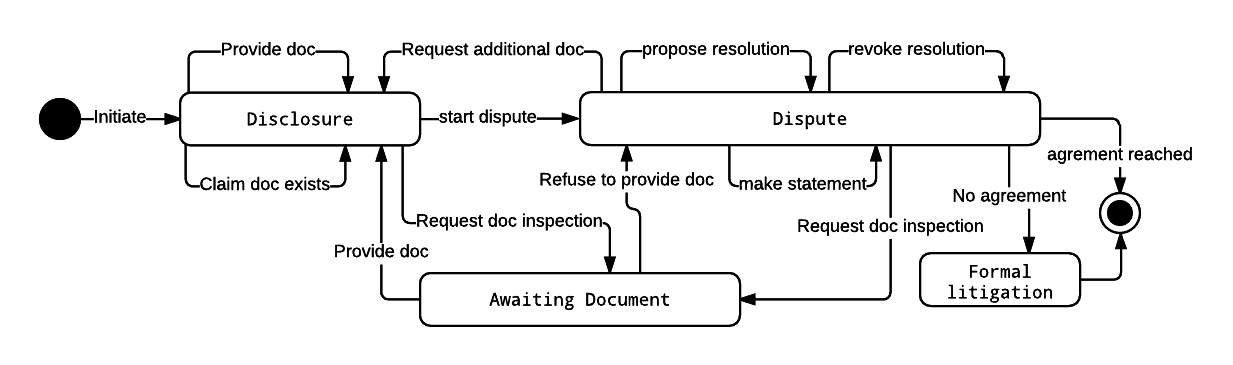
\includegraphics[width=1.0\textwidth]{./figures/adr_workflow.png}
    \caption{ADR Workflow}
    \label{fig:adr_workflow}
\end{figure}

\section{Formalising Disclosure} \label{sec:formalising_disclosure}
There are many different ways to perform disclosure, and depending on the type of ADR as well as the domain of the dispute, financial, civil etc, the process can vary. In civil litigation full disclosure is usually recommended, while in financial disputes the involved parties may choose not to disclose confidential information to the other party, but only to the intermediary. In this chapter we formally define how disclosure can be performed using blockchain technologies without a third party involvement based on the ADR workflow illustrated in figure \ref{fig:adr_workflow}.

Disclosure is merely the claim that a document exists, where the disclosing party has an obligation to produce the document should the other party request inspection of it. This is loosely based on UK civil procedure rules as defined in \cite{justice_gov:civil_procedure_rules}. To perform disclosure without the involvement of a third party, a disclosed document must provide three guarantees:
\begin{enumerate}
    \item{\textbf{Proof of existence:}} It must be possible for any of the involved parties to proof that a document existed at a certain time in the past. \label{itm:disclosure_document_objectives_existence}

    \item{\textbf{Proof of disclosure:}} It must be possible for any involved party to proof that a document was disclosed by another involved party. \label{itm:disclosure_document_objectives_disclosure}

    \item{\textbf{Secrecy against evesdropper:}} Secrecy of the document exchange must be guaranteed, that means that while eavesdroppers may be able to intercept that two parties are communicating, the identity as well as details of the interaction must remain secure. \label{itm:disclosure_document_objectives_evesdrop}

    \item{\textbf{Secrecy of confidential information amongs parties:}} It must be possible to obfuscate confidential information such that the counterparty will only know of it's existence and information that is willingly provided. It must also be possible to later on produce the confidential document in a verifiable manner. \label{itm:disclosure_document_objectives_confidential}

    \item{\textbf{Proof of identity of involved parties:}} It is desirable for each party to have the ability to proof the identity of the party that has disclosed documents for the purpose of possible follow up formal litigation processes. This is briefly investigated in chapter \ref{chapter:key_management}. 
\end{enumerate}
In order to meet the above mentioned objectives while remaining blockchain agnostic, a micro transaction framework is devised that is based on the definitions provided in the following sections:

\subsection{Definition of Document} \label{sec:definition_of_document}
A Document is defined as a composite of the document and cryptographic proofs to meet the objectives set out in the previous section. Formally a document is defined as the quadruple:
\begin{equation}
    \doc := (\keydocowner, \doctitle, x, S(\keydocowner^{-1}, (\keydocowner, \doctitle, x))) \mid x \in \{ E_{\{p,s\}}(\_, \content), \content\}
    \label{eq:disclosure_document}
\end{equation}
It consists of the public key of the disclosing party $\keydocowner$, a freetext title or description of the document $\doctitle$, $x$ which depending on the requirements is either the plaintext content $\content$ or the encrypted contents using either public or private key cryptography with a key of choice $E_{\{p,s\}}(\_, \content)$. The last component is a cryptographic signature using the private key of the disclosing party $\keydocowner^{-1}$ over the triple $(\keydocowner, \doctitle, \content)$.
In this work, documents openly disclosed are sent in plaintext, i.e. $x := m$ and for private documents that shall be withheld from inspection by the other party, symmetric key cryptography with a per-document key is used, i.e. $x := E_s(\keydocument, m)$. While there do exist more sophisticated mechanisms like multi party computation to securely share encrypted data with no one party knowing the full key, this is out of scope and considered future work.

\subsection{Definition of Acknowledgement} \label{sec:definition_of_acknowledgement}
While some ADR methods are private, meaning that nothing that happened in the process can be used outside or in later court cases, there do exist situations where it is desirable that it can be proven that a document was disclosed to a certain party. To this extent an acknowledgement is defined as the triple:
\begin{equation}
    \docack := (\keydocrecipient, \doc, S(\keydocrecipient^{-1}, (\keydocrecipient, \doc))
    \label{eq:disclosure_ack}
\end{equation}
where $\keydocrecipient$ is the public key of the recipient of the document, $\doc$ the document as per equation \ref{eq:disclosure_document}, and $S(\keydocrecipient^{-1}, (\keydocrecipient, \doc)$ a cryptographic signature using the private key $\keydocrecipient^{-1}$ to make proof the validity of the recipient.


\subsection{Definition of Receipt} \label{sec:definition_of_receipt}
A receipt is defined as the Chainpoint receipt generated from anchoring the document $\doc$ or the document acknowledgement $\docack$. To be precise, a cryptographic hash $H(x) \mid x \in \{\doc, \docack\}$ is anchored using the system described in \ref{sec:disclosure_anchor_data}. 
Following this process, there exist two types of ADR receipts, one for the document itself and one for the acknowledgement, formally a receipt is defined as a tuple
\begin{equation}
    \receipt := \begin{cases}
        (\docreceipt, \doc) & \textrm{if receipt for } \doc \\
        (\docackreceipt, \docack) & \textrm{if receipt for }  \docack
    \end{cases}
\end{equation}
where $\docreceipt$ is the Chainpoint receipt for the document $\doc$ and $\docackreceipt$ is the Chainpoint receipt for the document receipt acknowledgement $\docack$ generated by the anchoring system. The implemented system does not actually generate above receipt tuple but stores $\doc$ as well as $\docack$ if present in the blockchain as well as their anchoring receipts which can be obtained at any time. Typically involved parties would also back up the documents as well as receipts offline for future reference.

\subsection{Definition of the disclosure protocol}
The disclosure protocol can loosely be defined as a state machine with state
\begin{equation}
    S := \{\Receipt, \Docack, \Doc | \receipt \in \Receipt, \docack \in \Docack, \doc \in \Doc\}
    \label{eq:disclosure_state_machine}
\end{equation}
where $\Receipt$ is the set of all receipts, $\Docack$ the set of all document receipt acknowledgements and $\Doc$ the set of all documents and state transfer functions $\statetransferfunc_{add}$, $\statetransferfunc_{ack}$, $\statetransferfunc_{anchor}$ that modify the state of the system $S_t := \statetransferfunc_x(S_{t-1}, \_) \mid x \in \{add, ack, anchor\}$ and are formally defined as:
\begin{equation}
    \statetransferfunc_{add}(\{\Receipt, \Docack, \Doc\}, \doc) := \begin{cases}
        \{\Receipt, \Docack, \Doc \cup \doc\} & \textrm{if} \doc \not\in \Doc \\
        \{\Receipt, \Docack, \Doc\} & \textrm{if} \doc \in \Doc
    \end{cases}
    \label{eq:disclosure_state_transfer_add}
\end{equation}
\begin{equation}
    \statetransferfunc_{ack}(\{\Receipt, \Docack, \Doc\}, (\doc, \keydocrecipient, \keydocrecipient^{-1})) := \begin{cases}
        \{\Receipt, \Docack \cup \docack, \Doc\} & \textrm{if} \doc \in \Doc \\
        \{\Receipt, \Docack, \Doc\} & \textrm{if} \doc \not \in \Doc
    \end{cases}
    \label{eq:disclosure_state_transfer_ack}
\end{equation}
\begin{equation}
    \{\Receipt \cup \receipt, \Docack, \Doc\} := \statetransferfunc_{anchor}(\{\Receipt, \Docack, \Doc\}, x) \mid x \in \{\doc, \docack\}
    \label{eq:disclosure_state_transfer_anchor}
\end{equation}
Informally, $\statetransferfunc_{add}$ can be seen as preparing the document for anchoring, $\statetransferfunc_{ack}$ as the counter party acknowledging the receipt of the document and $\statetransferfunc_{anchor}$ as the anchoring system embedding the documents cryptographic hash into a transaction and generating a Chainpoint receipt.
The state machine describing the protocol for each document is illustrated in figure \ref{fig:disclosure_state_machine} where acknowledgement is optional depending on the use case. This protocol in combination with above definitions can be used to meet the objectives set in section \ref{sec:formalising_disclosure}, and how this is achieved is described next.

\begin{figure}
    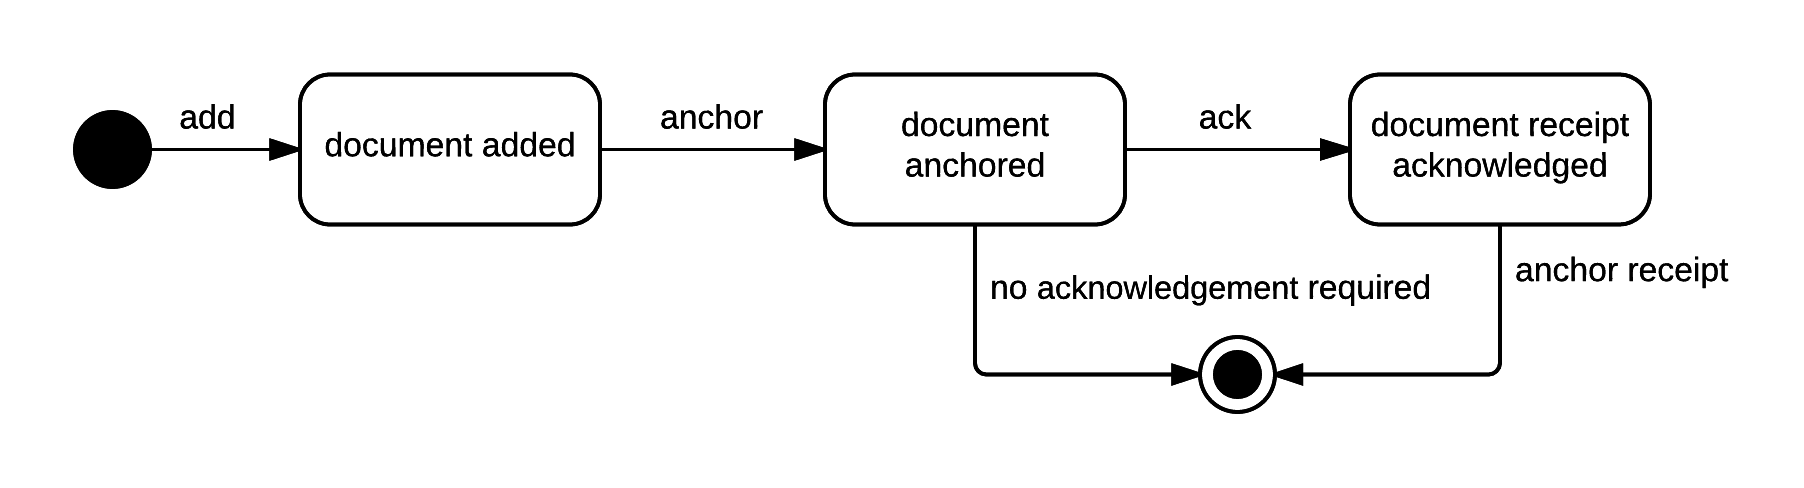
\includegraphics[width=1.0\textwidth]{./figures/disclosure_protocol.png}
    \caption{Disclosure protocol state machine}
    \label{fig:disclosure_state_machine}
\end{figure}

\subsection{Applicability of the protocol to defined objectives}
This section describes how a receipt $\receipt$ can be used to meet the objectives set for the system, in particular:
\begin{enumerate}
    \item{\textbf{Proof of existence:}} The Chainpoint receipts $\docreceipt$ and $\docackreceipt$ contain information about the transaction that contains $H(\doc)$ or $H(\docack)$ and can hence be used to proof that the document and the acknowledgement of it's receipt existed before the said transaction was generated and mined.
    \item{\textbf{Proof of disclosure:}} The document receipt acknowledgement $\docack$ contains a signature of the receiving party, proving that they have received the document $\doc$ included in the acknowledgement. The disclosing party then has the ability to proof that the acknowledgement is for the document provided.
    \item{\textbf{Secrecy against evesdropper:}} Assuming the communication channel between the opposing parties is not secure, then encrypting each document with it's unique, or alternatively a per dispute key provides secrecy against evesdroppers.
    \item{\textbf{Secrecy of confidential information amongst parties:}} As all documents can be encrypted with a secret key, it is easily possible to send a document to the other party while withholding the key, effectively proving that the document exists but not disclosing it's contents.\footnote{Shared key cryptography is a potential improvement to this approach but left for future research.}
    \item{\textbf{Proof of identity of involved parties:}} The outlined protocol provides no guarantees about the identity of parties behind the public keys, this problem is briefly investigated in chapter \ref{chapter:key_management}.
\end{enumerate}


\section{Tierion and the Chainpoint standard}
Tierion is by far not the only provider of blockchain based notary-like services, they are however one of the more sophisticated ones and to the best of our knowledge the only ones to have defined a public standard for blockchain receipts. Because of this standard as well as their popularity and flexible API the decision was made, to base the implementation of this system on their specification.

It is however important to note, that while Tierion as well as the open source library developed in this work do anchor documents into the blockchain, there is no association between the owner of the document and the document itself apart from the data stored in a database. In order to link an entity, or more precisely a public key, to the document anchored in the blockchain, it would be necessary for everyone who wants to anchor data into the blockchain to have their own account on every blockchain that the system integrates with as well as possess sufficient funds to pay for the transaction fees. In times where bitcoin transaction fees surged to ~5\$ this would be a very expensive and wasteful approach.

\section{Anchoring data into the Blockchain} \label{sec:disclosure_anchor_data}
In the first phase of this project, a system was developed that provides data storage capabilities as well as anchoring of all stored data records into a public blockchain. This system is based on the software offering of Tierion\footnote{\url{https://tierion.com}} and mimics their REST API. This system is intended to be eventually provided as an open source version of Tierions software system.

\subsection{Library Design}
Conceptionally, Tierion does two things. It provides a document management facility and a mechanism to anchor these documents as well as arbitrary sha256 hashes into the blockchain. These concepts drove the decision to break the library up into two stand-alone components, a document management part with a REST API as well as an anchoring API detailed in the following sections.

\begin{figure}
    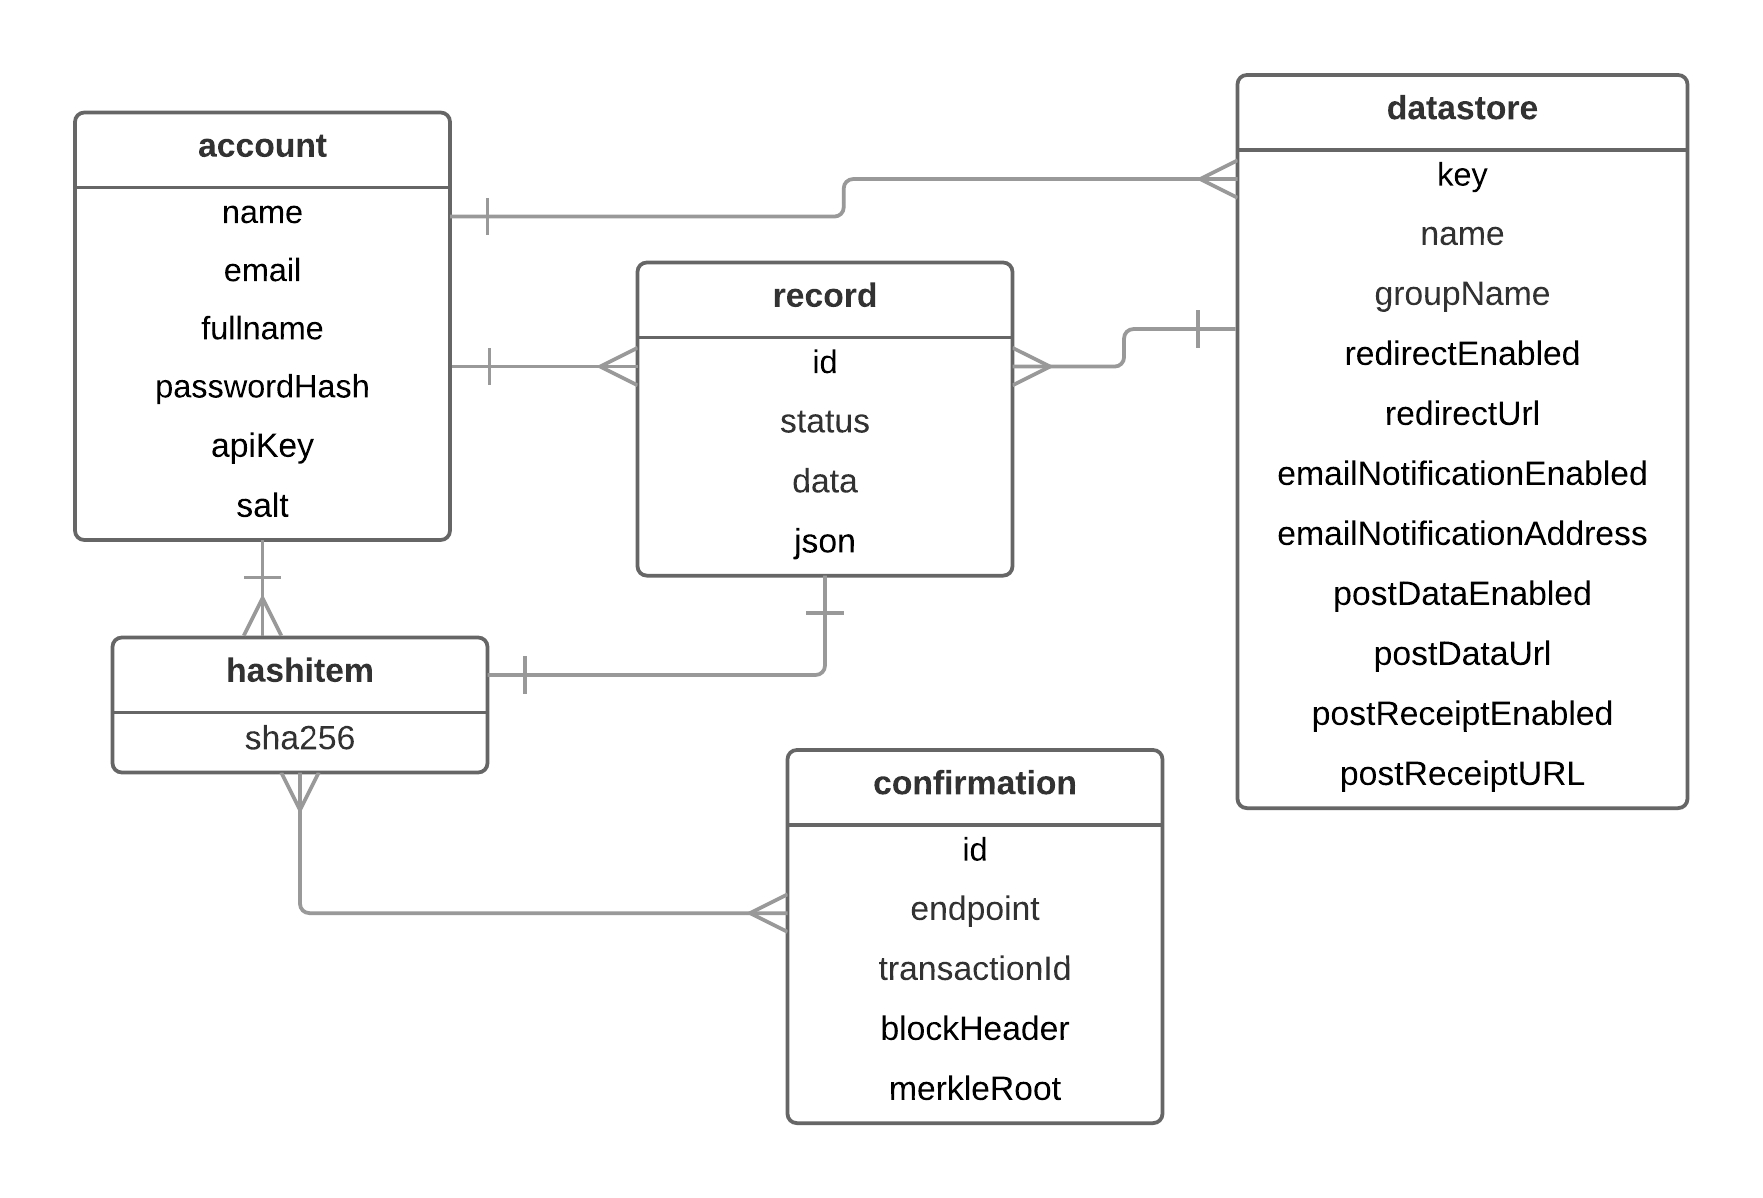
\includegraphics[width=1.0\textwidth]{./figures/tierion_db.png}
    \caption{OpenTierion Database Design}
    \label{fig:tierion_database_design}
\end{figure}

\subsection{Document management Component}
The document management component that is exposed via a REST API equivalent to the one defined by Tierion uses a database to store account data, documents as well as the information necessary to generate Chainpoint receipts. The database design is illustrated in figure \ref{fig:tierion_database_design} and the tables are defined as:

\begin{itemize}
    \item \textbf{account:} Holds information about the users account including login information, an api key and information required for a login token.

    \item \textbf{record:} Records in this context represent a document structured as json. The fields are equivalent to the ones defined by the tierion API.

    \item \textbf{datastore:} A Datastore can be seen as a collection of documents that allows to organize documents and set notifications for when certain actions occur on it.

    \item \textbf{hashitem:} A hashitem is a sha256 hash that is then anchored into the blockchain. It is possible to anchor a sha256 hash directly via a hashitem or anchor a record, where a sha256 hashitem is generated based on it's data.

    \item \textbf{confirmation:} Chainpoint at the time of writing supported two endpoints, Bitcoin and Ethereum. A Confirmation in this context represents information about the transaction the document was anchored in. Multiple confirmations in combination with the HashItem they are associated with hold the information required to build a chainpoint receipt.
\end{itemize}
In addition to the document management exposed to users, the library is designed in a way, such that one account is used per backend - more about backend integration in section \ref{sec:opentierion_backends} - to anchor multiple documents across multiple datastores and users. This is done via a periodic check for document age and the number of documents pending anchoring. Once either of these thresholds, which are configurable in the API are exceeded, all pending documents are put into a merkle tree and this merkle tree's root is then anchored into the blockchain and associated with the documents referenced in it.

\subsection{OpenTierion REST API} \label{sec:opentierion_rest_api}
The Tierion API is split into two separate REST APIs, a so called \texttt{Hash API} and a \texttt{Data API}. As compatibility with Tierion was one of the design goals, this open source implementation exposes an API mimicing this structure. Tables \ref{tab:opentierion_hash_api} and \ref{tab:opentierion_data_api} outline the API and operations supported by it. In addition to these APIs, a user API is exposed such that it is possible to manage user accounts via the API.

The Hash API is based on the specification on \url{https://tierion.com/docs/hashapi} and outlined in table \ref{tab:opentierion_hash_api}. Every operation on the hash API requires an access token to be supplied as the header \texttt{Authorization: Bearer <token>}. Tokens can be generated using the API as described in the specification table. The subscription component of the Tierion API was not implemented as part of this work and is left as a future improvement.
\begin{table}[!htbp]
    \begin{tabularx}{\textwidth}{| l l l X |}
        \hline
        \textbf{REST Endpoint} & \textbf{Type} & \textbf{Required fields} & \textbf{Description} \\
        \hline
        v1/auth/token & POST & username, password & Generates an auth token that is valid for one hour. Response includes the token, expiry time and a refresh token. \\

        v1/auth/refresh & POST & refreshToken & Generates a new auth token without supplying username and password again. \\

        v1/hashitems & POST & hash & Queues the hash provided for anchoring into the blockchains. \\
        \hline
    \end{tabularx}
    \caption{OpenTierion Hash API Spec}
    \label{tab:opentierion_hash_api}
\end{table}

The Data API is based on the specification on \url{https://tierion.com/docs/dataapi} and outlined in table \ref{tab:opentierion_data_api}. Every request to the Data API must include the header following header fields, where the api key can be obtained using the user API specified in table \ref{tab:opentierion_user_api}:
\begin{itemize}
    \item\texttt{X-Username: youremail@address.com}
    \item\texttt{X-Api-Key: YourAPIKeyGoesHere}
\end{itemize}
It is not required to supply auth credentials to create a user, to delete or query user information however it is required to supply the users email as well as the password as HTTP Basic auth credentials.

\begin{table}[!htbp]
    \begin{tabularx}{\textwidth}{| l l X X |}
        \hline
        \textbf{REST Endpoint} & \textbf{Type} & \textbf{Required fields} & \textbf{Description} \\
        \hline
		v1/datastores & GET & None & Retrieve all datastores for the current user \\

        v1/datastores/\textless id\textgreater & GET & None & Retrieve the datastore with the specified ID \\

        v1/datastores & POST & name & Create a new DataStore, please refer to online docs for more details. \\

        v1/datastores/\textless id\textgreater & PUT & None & Update the DataStore with the id specified, only supplied fields will be changed \\

        v1/datastores/\textless id\textgreater & DELETE & None & Delete the DataStore with the id specified. \\

        v1/records?\textless query\textgreater & GET & None & Retrieve records that match the query specified. Please refer to online docs for query syntax \\

        v1/records/\textless id\textgreater & GET & None & Retrieve the record with the ID specified. \\

        v1/record & POST & datastoreId & Create a new record associated with a datastore. All other fields will be treated as fields of the record. \\

        v1/records/\textless id\textgreater & DELETE & None & Delete the record with the id specified. \\

        \hline
    \end{tabularx}
    \caption{OpenTierion Data API Spec}
    \label{tab:opentierion_data_api}
\end{table}

\begin{table}
    \begin{tabularx}{\textwidth}{| l l X X |}
        \hline
        \textbf{REST Endpoint} & \textbf{Type} & \textbf{Required fields} & \textbf{Description} \\
        \hline
        v1/accounts & POST & name, email, full\_name, secret & Creates a new account \\
        v1/accounts/\textless name\textgreater & DELETE & None & Deletes the account \textless name\textgreater, requires HTTP basic auth with email and password  \\
        v1/accounts/\textless name\textgreater & GET & None & Retrieves account information including API key, requires HTTP basic auth with email and password \\
        \hline
    \end{tabularx}
    \caption{OpenTierion User API Spec}
    \label{tab:opentierion_user_api}
\end{table}

\subsection{Blockchain integration Component} \label{sec:opentierion_backends}
While the data management component allows users to create, manage and queue items for anchoring, the Blockchain integration component is required to actually perform the anchoring. When the library is instanciated, the integration component is registered with the data management component, and whenever documents are ready for anchoring due to them having been queued up for too long or the number of pending documents exceeding a configured threshold, this registered callback is called.

The library provides two main integrations, one for Bitcoin and one for Ethereum, detailed below. Each of these integrations is designed to work with a list of services that expose blockchain functionality. In the case of Ethereum two services were implemented, a web3 integration talking to a local Ethereum node as well as an integration with Etherscan\footnote{\url{https://etherscan.io/}} such that it is not required to run a local node. In case of bitcoin, a bitcoind integration was implemented to connect to a locally running node. Anchoring itself works very differently in Bitcoin than it does in Ethereum as detailed below.
\begin{itemize}
    \item \textbf{Bitcoin:} The bitcoin protocol was designed to work for the use-case of running a decentralised currency and it is not readily possible to supply arbitrary data to a transaction. As bitcoin transactions are basically a collection of inputs and outputs, and at least one valid output must be present in the transaction, a way to supply arbitrary data is to create one valid output to send the change back to oneself and additionally create an output with a pubkey script that can never be successfully evaluated and is as such an unspendable output. The pubkey script used for this purpose is called OP\_RETURN\footnote{\url{https://en.bitcoin.it/wiki/OP_RETURN}} and was introduced as a way to effectively burn bitcoins. The signing is done offline with the private key supplied to the integration library. If the private key supplied is a python function, then when a signature is required, the callback is called with the transaction as it's parameter such that integration with a hardware keystore is possible.

    \item \textbf{Ethereum:} As Ethereum was designed with the notion of contract execution via transactions, an Ethereum transaction already contains an arbitrary data field that is typically used to supply function arguments or contracts to the network. For this reason, anchoring an arbitrary hash is as easy as supplying the sha256 Merkle root as data in a transaction. Transactions are built locally and use the account/private key supplied in the library configuration. The private key supplied can either be a private key in which case the transaction will be signed locally using this private key, or a python function that gets called back with the transaction as an argument such that integration with a hardware keystore for security reasons is possible as well. Once the transaction is signed it is sent to the service and subsequently broadcast to the network. The returned transaction ID is then used to generate a Chainpoint receipt. It is worth noting that the account associated with the private key must have enough funds to pay the transaction fees.
\end{itemize}
As already mentioned earlier, the library will be open sources and made available on GitHub with more extensive documentation provided online.

\chapter{Key Management} \label{chapter:key_management}
In this chapter, a few possible approaches to Key Management are outlined as it is a requirement for the system to associate identity with keys. Due to the scope of this project, implementing any of these approaches is left for future research.

Wikipedia \cite{wiki:key_management} defines Key Management to be the management of cryptographic keys in a cryptosystem, including the generation, exchange, storage, use, destruction and replacement of keys on the user level. While this work does not focus on this aspect of the ADR system, it is important for a participant in the dispute to prove that another party has agreed to a certain resolution. As parties are only identified via their public keys, being able to prove that a public key represents a given entity is a requirement for this system. 

\section{Certificate Based Identification}
Certificate Authorities are a well established model used in the SSL standard. In this system there would be a set of trusted authorities that have the absolute trust of all parties in the system to not ever be corrupted and not make mistakes. This way, each public key would be associated with a Certificate signed by the CA, or another trusted party that holds a certificate signed by the CA essentially creating a so-called chain of trust. The main problem in this system is that the CA has to be incorruptible, and there exist plenty examples of CA's that issued invalid certificates in the context of SSL.

\section{Identity-Based Cryptosystems}
Initially proposed by Shamir \cite{shamir1984identity}, Identity-Based Encryption uses arbitraty public keys, allowing for the public key to be e.g. an email address, a phone number or another string identifying the entity behind the key. Using a central, trusted authority, private keys can then be derived from that arbitry string public key. The problem in this setup is that it depends on a central authority holding a private key that must be kept secret. These schemes have the advantage that they don't require a certificate, as the public key itself already acts as such. Boneh and Franklin \cite{boneh2001identity} and Sakai and Kasahara \cite{sakai2003id} propose IBE schemes for elliptic curves which could hence be used with blockchains.

\section{Cryptographically signed biometrics or video}
A different approach to the identity problem would be to require each participating party to record a video tape of themselves stating who they are and whom they represent, which they then cryptographically sign using their private key and share both, the signature as well as the video tape with the counter party. This way, it is possible to proof that the video tape was signed by the entity holding the private key associated with the public key used to verify the signature.

\section{Namecoin}
Namecoin\footnote{\url{https://namecoin.org/}} is a cryptocurrency, more precisely a fork of the bitcoin protocol, that provides a key-value type storage on a blockchain. Using the proof of existence guarantee a blockchain provides, it is possible to register the public key with an identity on the blockchain, essentially providing a globally unique association of the key. While this approach is interesting in it's simplicity, there needs to be some mechanism in place to ensure that the registered information is correct as it cannot be changed.

\section{Estonian e-Residency}
The last alternative outlined in this paper is the Estonian e-Residency. In 2014, Estonia launched an initiative to support electronic residency as a wider initiative to digitise the government. While e-Residency does not equal citizenship and hence does not include the right to enter the country, it does associate Identity with a cryptographic key, which can be used in a similar way to the Certificate-Based system, but with a government instead of a CA issuing these. \cite{estonia:eResidency}

\chapter{Dispute - Negotiation using Logic} \label{chapter:dispute}
In this chapter, the dispute phase as illustrated in figure \ref{fig:adr_workflow} is defined and a formal language as well as protocol that allows two parties to argue a dispute using blockchains instead of a neutral third party is designed. This chapter concludes with a design of a system that can provide negotiation support based on the formalism used and protocol designed.  

After discovery has been completed, and all documents made available, the involved parties enter the dispute phase as illustrated in figure \ref{fig:adr_workflow}. In traditional ODR systems, both parties use a third party service to act as a neutral intermediary that is usually used to keep the utility and constraints specified by either party secret. These systems are typically based on research in the well studief field of multi-agent negotiation. There exist a wide range of approaches and techniques to formulate as well as resolve disputes, Rahwan et al in \cite{Rahwan:2003:AN:1030328.1030332} categorize them as game theoretic, heuristic based and argumentation based. They also point out that neither approach suits all needs and there is no one type that fits all disputes. In this work, a combination of a game theoretic and argumentation based approach is designed. 

The following sections provide a formalism for a dispute using argumentation based approaches from \cite{Lodder:ORD_system_design}, \cite{Bellucci:2004:IAI:1032651.1033678}, \cite{Rahwan:2003:AN:1030328.1030332} as well as game theoretic ones as described in \cite{Susskind:Logic_of_mediating_values}, \cite{Ragone:2006:PAO:1124566.1124569}, \cite{Ragone2008}, \cite{Wooldridge:2000:LN:3006433.3006516}, \cite{Chevaleyre:2005:NOS:1082473.1082518}.

\section{Definition of a Dispute}
Disputes come in a lot of varieties, and it is not possible to define one model that is a perfect fit for all of them, there are however some general assumptions as to how a typical dispute works which are used as basic assumptions for this work. According to \cite{Susskind:Logic_of_mediating_values} a typical dispute follows four logical assumptions which are also consistent with the requirements posed on an ODR system as defined in \cite{Lodder:ORD_system_design} as:
\begin{enumerate}
    \item{disputants know what they want and have a fallback plan, a "Best Alternative To Negotiated Agreement" - BATNA}
    \item{Even if their demands are much higher than the BATNA, they're eager to negotiate a mutually beneficial deal which should be supported by the negotiation tool}
    \item{negotiate on issues and eventually reach a middle ground, that in the ODR setting is typically a solution proposed by the system using compensation/trade-off strategies}
    \item{a binding, written agreement is formalised and signed by all participating parties.}
\end{enumerate}
It is important to note that identifying the BATNA is a hard problem on it's own and is not addressed in this thesis. For the purpose of this work, a dispute is defined as having Documents, Statements, Demands and Offers, as well as utilities that define the importance of demands and offers such that the system can value trade-offs and recommend solutions to the involved parties. In addition to the elements defining a dispute, the following properties are ideally all exhibited by system.
\begin{itemize}

    \item{\textbf{Offline:}} The system should not require both parties to be available at the same time and effectively provide a way to make a statement, demand or offer that can later on be addressed by the other party.

    \item{\textbf{Proof of existence:}} Either party needs to be able to proof that the other party has either specified demands that were met by the other party, or proposed an offer that meets the demand, such that in case of either party attempting further formal litigation, there exists a proof of resolution of the dispute.

    \item{\textbf{Secrecy of utility and preference:}} It usually isn't in the interest of either party that the opposing side knows their utility function. The system should hence provide a way for the utility function to be either fully or partially private while still providing both parties a way to resolve the dispute.

    \item{\textbf{Independence of third party:}} It must be possible for the system and the participants to progress a dispute without the need for a neutral third party.

    \item{\textbf{Possibility of involving a third party:}} It is desirable to be able to involve a third party (Facilitator, Mediator, Arbitrator) in case the dispute comes to a state where no progress is made. The third party should be able to get access to all interactions that have happened between disputing parties.

    \item{\textbf{Incentivise agreement:}} The system should have a mechanism in place that encourages the involved parties to reach a consensus, as otherwise they could benefit from delaying the process indefinitely.

    \item{\textbf{Proof of identity of involved parties:}} Both parties need to be able to proof the identity of the other side in order to legally enforce that they act on the accepted negotiated resolution.

\end{itemize}

\subsection{Formal definition of the dispute framework} \label{sec:formalising_dispute}
A dispute can be seen as a negotiation over issues between two parties and can formally be defined in the sense of a Bargaining Game as pioneered by Nash \cite{Nash:bargaining} and expanded on by Rubenstein \cite{Rubenstein}, that enables the system to find a solution that represents a Nash Equilibrium or is Pareto optimal. This definition uses a propositional logic extended with concrete domains $\Proplang$ as defined by \cite{Ragone2008} as well as borrows from \cite{Lodder:ORD_system_design}, \cite{DBLP:journals:corr:ZhangZ14a}, \cite{Bellucci:2004:IAI:1032651.1033678} and \cite{Hemaissia:2007:MMN:1329125.1329314}.
In this work, parties in a dispute can argue issues traceably using a mechanism similar to statements described in \cite{Bellucci:2004:IAI:1032651.1033678} and use $\Proplang$ to formalise their demands or offers. Demands and offers are made up of two types of issues, propositional atoms $\propatom \in \{true, false\}$ and variables $\propvar \in \Propdom_{\propvar}$ where $\Propdom_{\propvar}$ is the numerical domain associated with the variable. Variables are constrained by their domain and a comparison with a constant. These definitions allow to formalise demands and offers like \texttt{resideWithWife$\wedge$(childSupport$\geq$2500)} representing the demands that the wife wants the children to reside with her and child support payments of at least £2500 per month. Additionally conditional demands like \texttt{houseToWife$\Rightarrow$(childSupport$\leq$1000)} representing the fact that if the family home is given to the wife, then child support payments would be less can be formulated as well. For completeness, formal definitions from \cite{Ragone2008} and \cite{Baader:1991:SIC:1631171.1631239} for the above are provided next.

\begin{itemize}
    \item
        \textbf{Concrete Domains:}\cite{Baader:1991:SIC:1631171.1631239} A concrete domain $\Propdom$ consists of a finite set $\Delta_{\Predicate}(\Propdom)$ of numerical values, and a set of predicates $\Predicate(\Propdom)$ expressing numerical constraints on $\Propdom$.

        Predicates are always binary operators $\Predicate(\Propdom) := \{\geq, \leq, >, <, =, \neq\}$ with their second argument being a constant in the domain $\Delta_{\Predicate}(\Propdom)$, the domain can represent amounts of money, weekdays, colours etc depending on the requirements\cite{Ragone2008}.

    \item
        \textbf{The Language $\Proplang$:}\cite{Ragone2008} Let $\Propatom$ be a set of propositional atoms, and $\Propvar$ a set of pairs $\langle\propvar, \Propdom_{\propvar}\rangle$ each made of a feature name and an associated concrete domain $\Propdom_{\propvar}$, and let $k$ be a value in $\Propdom_{\propvar}$. Then the following formulas are in $\Proplang$:
        \begin{enumerate}
            \item every atom $\propatom \in \Propatom$ is a formula in $\Proplang$
            \item if $\langle \propatom, \Propdom_{\propvar} \rangle \in \Propvar, k \in \Propdom_{\propvar}$, and $c \in \{\geq, \leq, >, <, =, \neq\}$ then $(\propvar ck)$ is a formula in $\Proplang$
            \item if $\psi$ and $\varphi$ are formulas in $\Proplang$ then $\neg\psi$, $\psi \wedge \varphi$ are formulas in $\Proplang$\footnote{Additionally: $\psi \vee \varphi := \neg(\neg\psi\wedge\neg\varphi)$, $\psi\Rightarrow\varphi := \neg\psi\vee\varphi$ and $\psi\Leftrightarrow\varphi := (\psi\Rightarrow\varphi)\wedge(\varphi\Rightarrow\psi)$}
        \end{enumerate}

    \item
        \textbf{Interpretation and Models:}\cite{Ragone2008} An interpretation $\Interpretation$ for $\Proplang$ (denoted as a superscript .$^{\Interpretation}$ on it's arguments) is a function that maps each atom in A into a truth value $\propatom^{\Interpretation} \in \{true, false\}$, each feature name $\propvar$ into a value $\propvar^{\Interpretation} \in \Propdom_{\propvar}$, and assigns truth values to formulas as follows:
        \begin{itemize}
            \item $(\propvar ck)^{\Interpretation} = true$ iff $\propvar^{\Interpretation}$ is true in $\Propdom_{\propvar}$ and false otherwise
            \item $(\neg\psi)^{\Interpretation} = true$ iff $\psi^{\Interpretation} = false$, $(\psi\wedge\varphi)^{\Interpretation} = true$ iff both $\psi^{\Interpretation} = true$ and $\varphi^{\Interpretation} = true$, according to truth tables for propositional connectives.
        \end{itemize}

        The notation $\Interpretation\models\varphi$ denotes the fact that $\Interpretation$ is a model for $\varphi$ meaning that it assigns $true$ to $\varphi$. $\Interpretation$ is said to be a model for a set of formulas if it assigns true to every formula in the set.
\end{itemize}
In addition to the formalisation for issues, parties must be able to provide statements to either back, or respond to issues and demands. For the purpose of this work the notion of a statement, based on \cite{Bellucci:2004:IAI:1032651.1033678}, is defined to allow for traceable communication. Formally there are two types of a statement $\statement \in \Statement$ made by a party $\party \in \Party$ containing freetext $\statementtext$, where $\Statement$ is the set containing all statements and $\Party$ the set containing all $\Numparties$ parties participating in the dispute. The two are defined as:
\begin{equation}
    \statement_a(\party, \statementtext, \alpha) \mid \alpha \in \Propvar \cup \Propatom \wedge \alpha \neq \varnothing
    \label{eq:initial_statement}
\end{equation}
\begin{equation}
    \statement_a(\party, \statementtext, \statement_b) \mid a \neq b
    \label{eq:initial_statement_s}
\end{equation}
Using these definitions, it is possible to provide statements based on issues expressed as atoms or variabes as well as statements based on earlier ones and they can be classified as the five distinct types:
\begin{enumerate}

    \item \textbf{Supporting/Responding statement on issue}: A statement, referencing an issue is called a supporting statement, if it is raised by the party benefiting from the demand and a responding one if it is raised by the party hurt by the issue. Formally this could be defined by attaching a label to each atom $\propatom$ and variable $\propvar$ in the language $\Proplang$, but it is not technically necessary to make this distinguishment for the purpose of this work.
        \begin{equation*}
            \statement(\party, \statementtext, \alpha) \mid \alpha \in \Propvar \cup \Propatom \wedge \alpha \neq \varnothing
            \tag{\ref{eq:initial_statement} revisited}
        \end{equation*}

    \item \textbf{Supporting statement on statement:} Supporting statements to prior ones are defined as responses to an earlier statement made by the same party:
        \begin{equation}
            \statement_a(\party_i, \statementtext, \statement_b(\party_j, \statementtext)) \mid i = j \wedge a \neq b
        \end{equation}

    \item \textbf{Responding statement on statement:} Responding statements to prior ones are defined as responses to an earlier statement made by an opposing party:
        \begin{equation}
            \statement_a(\party_i, \statementtext, \statement_b(\party_j, \statementtext)) \mid i \neq j \wedge a \neq b
        \end{equation}

    \item \textbf{Concluding statement on statement:} As a sequence of statements can be interpreted as a discussion on a certain topic, it is readily obvious that there needs to be a mechanism to conclude the discussion. These concluding statements are defined as:
        \begin{equation}
            \statement_a(\party_i, \varnothing, \statement_b(\party_j, \statementtext)) \mid a \neq b
        \end{equation}
\end{enumerate}

Building on above definitions, a set $\Statement'$ of unconcluded statements is defined as $\Statement' := \{\statement_a \in \Statement \mid \not\exists \statement_b \colon \statement_b(\_,\_,\statement_s)\}$ which is used to define an agreement.


\subsection{Formal definition of Resolution/Agreement} \label{sec:agreement}
A resolution or agreement to a dispute is defined as an interpretation $\Interpretation$ that assigns $true$ to the formulas $\demand$ and $\offer$ representing the demand and offer in combination with an ontology $\Ontology$ represented as a set of formulas in $\Proplang$ describing the domain of the dispute\footnote{An example formula in the ontology could be \texttt{resideWithWife$\Leftrightarrow\neg$resideWithHusband} or \texttt{DiscloseWifeUnfaithfulProof1$\Rightarrow$wifeCheated}}, formally\cite{Ragone2008}:
\begin{itemize}
    \item \textbf{Demand:} A demand is a formula $\demand$ in $\Proplang$ such that $\Ontology \cup \{\demand\}$ is satisfiable.
    \item \textbf{Offer:} An offer is a formula $\offer$ in $\Proplang$ such that $\Ontology \cup \{\offer\}$ is satisfiable.
    \item \textbf{Agreement:} A possible resolution to the dispute is defined as the set of all Interpretations $\Deal$ satisfying the demand as well as the offer in combination with the ontology $\{\Interpretation \mid \Interpretation \models \Ontology \cup \{\offer, \demand\}\}$. An agreement is then defined as a deal $\deal \in \Deal$ that both parties accept iff $\Statement' = \emptyset$
\end{itemize}


\section{Dispute Protocol and Domain Specific Language}
Wooldridge and Parsons \cite{Wooldridge:2000:LN:3006433.3006516} provide a definition of a negotiation meta-language which is an equivalent idea and the basis to the domain specific language, DSL, defined in this chapter and denoted as $\Metalang$. The protocol is designed as a repeatable one-shot negotiation with a reference to previous rounds of the game. It is worth noting that the protocol designed simply allows the two parties to negotiate using a blockchain, but does not provide any success guarantees or support that a third party like a Mediatior would otherwise provide. In section \ref{sec:negotiation_support} negotiation support without a third party is investigated.

\begin{figure}
    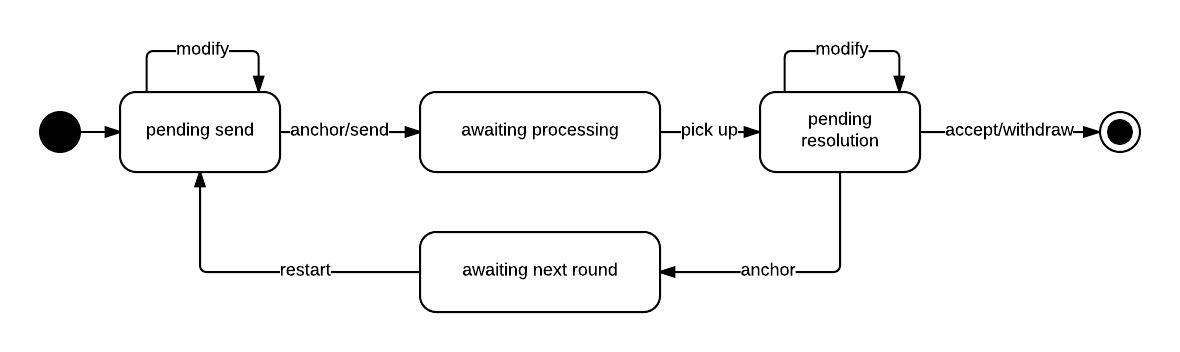
\includegraphics[width=\textwidth]{./figures/adr_dispute.png}
    \caption{High-level dispute protocol}
    \label{fig:adr_dispute}
\end{figure}

\begin{table}
    \centering
    \begin{tabularx}{\textwidth}{|l X|}
        \hline
        \textbf{Operation} & \textbf{Description} \\
        \hline
        $ref(h)$ & Indicate that this document is a continuation of the document identified by hash $h$ \\
        $disclose(\party, \receipt)$ & Party $\party$ states they have disclosed a document identified by a receipt $\receipt$ \\
        $ontology(\party, \Ontology)$ & Ontology $\Ontology$ provided by party $\party$. If both parties provide ontologies they are combined \\
        $constraint(\party, \varphi)$ & Constraint provided by party $\party$, It is allowed to specify multiple constraints. Depending on the party, the constraints are either demands or offers as defined in section \ref{sec:formalising_dispute} \\
        $state(\party, \statement)$ & Plain text statements (equation \ref{eq:initial_statement}) made by party $\party$ \\
        $accept(\party, \Interpretation)$ & Indicate that party $\party$ accepts interpretation $\Interpretation$ \\
        $withdraw(\party)$ & Indicate that party $\party$ withdraws from the negotiation \\
        \hline
    \end{tabularx}
    \label{tab:dsl_operations}
    \caption{Valid operations of the DSL $\Metalang$}
\end{table}

The DSL has to allow parties to specify they have disclosed documents, formalise the demands or offers, argue for or against those as well as accepting or rejecting a resolution. Valid operations $\metaop \in \Metalang$ are defined in Table \ref{tab:dsl_operations}. In the dispute protocol, illustrated in figure \ref{fig:adr_dispute} a party initiates a dispute by creating a document describing the dispute using $\Metalang$. When a party has finished formalising their demands, the document is cryptographically signed, anchored into the blockchain and made available to the other party. They then pick up the document and are faced with three options. They can either accept the demands as they are by providing an interpretation $\Interpretation$ that satisfies the constraints defined by the other party which concludes the dispute as long as an agreement as defined in section \ref{sec:agreement} is reached, they can choose to expand the document with their own operations and use a game theoretic approach to get a valid interpretation they can then accept, or they expand the document with statements and constraints such that no agreement can't be reached. In this case, the initiating party takes the document, adds a reference to the document specifying the system of constraints and statements that cannot be resolved and the process starts again with a modified set of constraints.

In order to guarantee consistency, the implementation guarantees that statements, and disclosed documents cannot be removed from the systems state, the ontology is always consistent and that a party is only allowed to modify their own constraints and ontology items. Another safety element is that once a party has finished modifying the system, the document is cryptographically signed before being sent to the other party such that it is possible to verify the authenticity of the demands.





%A simple example conversation between a Husband and a Wife in a marital dispute could then look something like:
%$\\s_0(W, “\textnormal{I want child support payments}”) \\
%s_1(H, "\textnormal{I'm not paying more than £500 a month}", s_0) \\
%s_2(W, \varnothing, s_1)$

%These discussions and issues are then translated into a propositional language formally defining the demands. In order for this document to be self contained, the definitions of \cite{Ragone2008} are outlined next and subsequently used to define the protocol used between the parties define demands and resolve them.



\section{Negotiation support and Game theoretic view} \label{sec:negotiation_support}
Many ODR systems provide negotiation support to identify the importance of certain issues to the parties, typically defined via utility functions as well as a mechanism to suggest a resolution to the dispute. While in \cite{Bellucci:2004:IAI:1032651.1033678} the system attempts to distribute resources based on trade-off maps, other approaches like \cite{Ragone:2006:PAO:1124566.1124569} use propositional logic as outlined in section \ref{sec:formalising_dispute}. In general all these approaches are based on the Bargaining game defined by Nash \cite{Nash:bargaining} and expanded on by Rubenstein \cite{Rubenstein} and attempt to find a Nash Equilibrium or a Pareto optimal outcome for both parties based on their constraints and utilities. All systems that provide negotiation support in a bargaining context, use third a neutral party, typically a software system, that has a complete view of the world, all the constraints of both parties as well as the utility functions they define such that they can calculate a solution to the problem without parties finding out about the constraints and utilities of the other ones. In the context of this work, the goal is to eliminate the need for a third party and in this section an approach is developed, that attempts to solve this issue. To this extend the following requirements are addressed:
\begin{itemize}
    \item\textbf{Offline:} A party should be able to specify their utilities, constraints etc, anchor the document and then not be online for the other party to progress the dispute. In order to support this, all the information required has to be available to the other party. The protocol in combination with the formalism from section \ref{sec:formalising_dispute} itself allows for that to happen. Using the approach of \cite{Ragone2008} of converting the system defined over the propositional language $\Proplang$ into an integer linear program, using utility functions over propositional atoms as well as variables over a concrete domain, an interpretation $\Interpretation$ satisfying the system can be found.

    \item\textbf{Secrecy of utility:} The utilities should not be visible to the other party. This is not easily achievable given this system as the linear program requires the utility function to be available for the optimization to run. Ragone et al \cite{Ragone2008} define a MAX-SUM-MBN that yields a Pareto optimal solution as a maximization problem over the sum of utilities of both parties, which for obvious reasons requires the utility functions to be known.

    \item\textbf{Secrecy of constraints:} The constraints should not be visible to the other party, which can be achieved using multi-party computation. Using the transformation based approach defined by \cite{Mangasarian2012} and expanded upon by \cite{Li2013} we can apply a linear transformation to the constraints of the linear problem and hence obfuscate the constraints defined using a privately held matrix $B$ and $D$ that is only known to the party that defined the constraints. This way it is possible to combine the two sets of constraints and find a valid $\Interpretation$ in the transformed space. While ILP problems are NP-Hard\footnote{In the general case, ignoring special cases} and hence calculating a solution to a large problem is expensive, a party in possession of the transformed constraint set can probe the system by attempting to solve it with different constraints, effectively figuring out the constraints of the counterparty using brute-force. More about this problem later.

    \item\textbf{Provability:} It must be provable to either party that the constraints defined are indeed valid and that the solution meets the constraints, which is trivially true. If the transformed linear program is signed and shared, then any solution to this problem is guaranteed to be a solution to the constraints specified by the other party.
\end{itemize}
This design leaves three problems partially unsolved, secrecy of utility functions, secrecy of constraints and verifiability by a third party. To this extent secrecy of utility functions is ignored in this work and all issues are considered equally important with a pre-defined linear utility on variables in the language $\Proplang$. This way valid solutions to the constraints can be found while the true utility is secret. Introducing an extra step into the protocol, which is manually accepting an interpretation $\Interpretation$ by both parties, solutions can be rejected if their utility is not high enough. The next problem is secrecy of constraints. While it is impossible for a part to learn their counterparties constraints directly, they can probe them using brute force. For large systems this is probably intractable as ILP solving is in general NP-Hard, yet it is a problem that shouldn't be ignored. The last problem is that because everything that's anchored in the blockchain is a hash of the document, only parties that have received a copy of the original document can participate and/or verify the dispute. While this is not a direct issue, it could be a desirable property to have a central monitor that is able to verify that a dispute has been resolved. These problems are left open for future research and are briefly addressed in section \ref{sec:future_work}.


\section{System design}

\chapter{Conclusion and Future Work}

\section{Conclusion} \label{sec:conclusion}

\section{Future Work} \label{sec:future_work}



\bibliographystyle{unsrt}
\bibliography{bibliography}
\end{document}
